% don't remove the following lines, and edit the definition of \main if needed
\documentclass[../report.tex]{subfiles}
\providecommand{\main}{..}
\IfEq{\jobname}{\currfilebase}{\AtEndDocument{\biblio}}{}
\IfEq{\jobname}{\currfilebase}{%file for shortcuts

\newcommand{\nch}{\ensuremath{N_{\mathrm {ch}}\xspace}}
\newcommand{\Ncoll}{\ensuremath{N_{\mathrm {coll}}}}
\newcommand{\Npart}{\ensuremath{N_{\mathrm {part}}}}
\newcommand{\dNdeta}{\mathrm{d}N_\mathrm{ch}/\mathrm{d}\eta}
\newcommand{\snn}         {\ensuremath{\sqrt{s_{\mathrm {NN}}}}}
\newcommand{\kT}          {\ensuremath{k_{\mathrm {T}}}}

\newcommand{\pp}          {pp}
\newcommand{\pPb}         {pPb}
\newcommand{\pA}          {pA}
\newcommand{\PbPb}        {PbPb}
\newcommand{\AuAu}        {AuAu}
\newcommand{\CuCu}        {CuCu}
\newcommand{\pAu}         {pAu}
\newcommand{\dAu}         {dAu}
\newcommand{\lsim}        {\,{\buildrel < \over {_\sim}}\,}
\newcommand{\gsim}        {\,{\buildrel > \over {_\sim}}\,}
\newcommand{\co}[1]       {\relax}
\newcommand{\nl}          {\newline}
\newcommand{\el}          {\\\hline\\[-0.4cm]}}{}
% until here

\emergencystretch=1em
\raggedbottom

\begin{document}

\section{Emergence of hot and dense QCD in small systems}

\textbf{Coordinators}: Jan Fiete Grosse-Oetringhaus (CERN) and Constantin Loizides (Oak Ridge National Laboratory) 
\linebreak
\textbf{Contributors, not yet sorted alphabetically, not complete}:
Naghmeh Mohammadi (CERN), 
Aleksi Kurkela (CERN), 
Christian Bierlich (University of Copenhagen), 
Bjoern Schenke (Brookhaven National Lab), 
Alexander Kalweit (CERN),
Mingliang Zhou (Stony Brook University),
Maxime Guilbaud (CERN),
Jiangyong Jia (Brookhaven National Lab), 
Cvetan Cheshkov (CNRS),
Elena Bruna (),
Henrique Zanoli (),
Peter Jacobs (LBNL),
Filip Krizek (),
Michael Weber (),
Ran Bi (),
Kaya Tatar (),
Yen-Jie Lee ()

\label{sec:smallsyst}

In the program of proton--proton collisions at the LHC, the main effort is focused on hard processes which are embedded in an underlying event consisting of a large number of soft low-$p_\perp$ particles. The underlying event is subtracted using models, such as PYTHIA~\cite{Sjostrand:2014zea} or HERWIG~\cite{Bellm:2015jjp}, based on essentially free streaming of the produced particles, supplemented in some cases with a non-perturbative string fragmentation picture~\cite{Andersson:1983ia} to model the non-perturbative soft particle production.  

In the past years at LHC, during run 1 and 2, this picture was challenged by several observations that qualitatively differ from the model expectations and can not be accommodated by tuning of the existing models used to describe the underlying event~\cite{Fischer:2016zzs}.
The first such observation was the unexpected discovery in 2010 of azimuthal correlations of final-state hadrons in very high multiplicity proton--proton collisions.\footnote{Details and experimental references are given in Sect.~\ref{sect:smallsystems_historicoverview}.} These persist even at large separation in rapidity surrounding the jet-like peak. A few years later, a similar observation was made in high multiplicity proton--lead collisions. By subtracting the jet-like contribution in proton--lead collisions, a second long-range rapidity correlation back-to-back in azimuth to the first observed correlation was extracted. Even later, the procedure was adapted to proton--proton collisions, allowing one also to extract also two long-range contributions in high-multiplicity proton--proton collisions. Under certain assumptions even lower multiplicity proton--proton collisions show the same features. With these observations the reminiscence of small and large collisions systems with respect to azimuthal correlations has been clearly demonstrated.
The second observation was that of enhanced production of multi-strange hadrons in high-multiplicity proton-proton collisions extending the discrepancy from final state particle kinematics to include also hadrochemistry. 
These observations have shed a different light on the study of heavy-ion phenomena in proton--proton and proton--lead collisions. Initially, these collisions were thought of as reference for the effects observed in lead--lead collisions. Instead their study has become a field on its own with significant interest in both, the heavy-ion and the high-energy physics community.

In ultrarelativistic nucleus--nucleus collisions, ranging from early SPS experiments at CERN through the Relativistic Heavy-Ion Collider (RHIC) at Brookhaven National Laboratory (BNL) to LHC, these qualitative observations have been interpreted as signs of formation of a droplet of thermalized Quark--Gluon Plasma. The long-range azimuthal correlations, and in particular their lowest harmonic component $v_{\rm{2}}$, have been used in combination with relativistic fluid-dynamical modeling to constrain the material properties of the plasma.  The striking result from RHIC was that the plasma formed in the central nucleus--nucleus (\AuAu) collisions flows as a liquid nearly without dissipation such that its specific viscosity $\eta/s$ -- quantifying the dissipative properties of the medium -- was found to be smaller than that of any other known substance. The inferred value of the specific shear viscosity $\eta/s\sim 0.07-0.16$ \cite{} was found to be significantly smaller than the expectation from perturbative QCD and other quasiparticles models and closer to the expectation of holographic model calculations of strongly coupled (maximally supersymmetric $\rm{N}=4$) gauge theories in the limit of large number of colors $N_c \rightarrow \infty$. These models can be seen as models of fluids with minimal dissipation allowed by basic principles of quantum mechanics thus giving rise to the paradigm of Quark--Gluon Plasma as a perfect liquid. The models of perfect fluid do not have a quasiparticle structure, and as such they are incompatible with free streaming. Therefore, the observation of fluid-like signatures as a small modification of free streaming evolution in small systems also challenges the perfect fluid paradigm. 

There are several theoretical pictures that have been suggested to explain the smooth onset of signals of collectivity in small systems. The proton--proton event generators have been supplemented on the one hand with elements describing string fragmentation in dense medium (DIPSY) to address the hadrochemistry and on the other hand with final-state interactions between the fragmenting strings to account for the final-state kinematical correlations~\cite{Bierlich:2017vhg}. 
The models of perfect fluid have been brought to their extreme and applied down to proton--proton collisions~\cite{Weller:2017tsr,Aidala:2018mcw} suggesting a formation of a nearly perfect liquid even in the smallest collision systems. Furthermore, pQCD based saturation models can describe the emergence of $v_{\rm{2}}$. In these models the final-state azimuthal correlations can arise either from the intrinsic correlations in the nuclear wave function (initial-state correlations) as correlated anisotropic particle production or as a final-state interaction after the initial particle production. 
A question remains to what extent these different models are describing qualitatively different physical phenomena or to what extent they are different prescriptions of the same underlying physics of final-state interactions. Transport theory, which can describe microscopic interactions but in the limit of large number of final-state interactions has a coarse grained effective description in terms of fluid dynamics has the potential to bridge the gap between the small systems, where final-state interactions act as small modification to the free streaming evolution, and central nucleus--nucleus collisions where the final-state interactions bring the matter to the fluid-dynamical limit. 

The experimental program in the large intermediate region --- spanning from mid-central \PbPb and \XeXe collisions, through \pPb collisions down to minimum-bias \pp collisions (and possibly even very high multiplicity e$^{+}$e$^{-}$ and e-p events) --- offers a possibility to reconcile the difference in the two limits by proving a setup where the microscopic final state interactions that lead in central \PbPb collision to the formation of QGP may be studied in isolation in the limit of small number of final-state interactions.  

The suggested theoretical pictures may have implications for high energy physics analyses, which depend on reliable models of the underlying event. As an example, it has been recently shown that the discussed long-range correlations are also present in the underlying event of $Z$-tagged \pp collisions. As the usual models used to describe the underlying event fail, even qualitatively, to describe this, better descriptions of collective effects in small systems are also vital for improving understanding in high-energy physics analyses.\todo{this paragraph can be improved}

The main experimental task in future years is twofold: Firstly, a detailed characterization of the similarities and differences in the overlap region between \pp, \pPb and \PbPb collisions, and secondly, the study of the onset of the observed effects.\todo{extend and merge with discussion on why pp and pPb are needed}

\todo{This chapter is structures as follows:}

\subsection{Historic overview}
\label{sect:smallsystems_historicoverview}
% Comments wrt initial LHC program

\afterpage{%
\begin{landscape}
\begin{table}[h!]
\begin{center}
  \small
  \begin{tabular}{p{5cm}|p{3.6cm}|p{3.6cm}|p{3.6cm}| p{3cm} }
    Observable or effect                 & PbPb                                          & pPb (high mult.)                  & pp (high mult.)                         & Refs.\\
    \hline
    \hline
    Low $\pT$ spectra (``radial flow'')  & yes                                             & yes                                & yes                            & \cite{Abelev:2012wca,Abelev:2013vea,Chatrchyan:2013eya,Chatrchyan:2012qb,Andrei:2014vaa,Abelev:2013haa,Acharya:2017dmc,Adam:2016bpr,Adam:2015vsf,Adam:2017zbf} \el
    Intermed.\ $\pT$ (``recombination'') & yes                                             & yes                                & yes                            & \cite{Andrei:2014vaa,Abelev:2013xaa,Abelev:2013haa,Abelev:2014uua,Khachatryan:2016yru,Adam:2015jca,Adam:2016dau,Adam:2017zbf} \el
    Particle ratios                      & GC level                                        & GC level except $\Omega$           & GC level except $\Omega$       & \cite{Adam:2016emw,Adam:2016bpr,Adam:2015vsf,ABELEV:2013zaa} \\
    Statistical model                    & $\gamma^{\rm GC}_s=1$, 10--30\%                   & $\gamma^{\rm GC}_s\approx1$, 20--40\%  & $\gamma^{\rm C}_s<1$, 20--40\%  & \cite{Floris:2014pta,Adam:2015vsf,ALICE:2017jyt} \el
        HBT radii ($R(\kT)$, $R(\sqrt[3]{\nch})$)        & $R_{\mathrm{out}}/R_{\rm side}\approx1$& $R_{\rm out}/R_{\rm side}\lsim1$         & $R_{\rm out}/R_{\rm side}\lsim1$       & \cite{Adam:2015vna,Adam:2015vja,Abelev:2014pja,Adam:2015pya,Aamodt:2011kd,CMS:2014mla,Acharya:2017qtq,Aaboud:2017xpw} \el
       Azimuthal anisotropy ($v_n$)\nl 
    (from two particle correlations)                   & $v_{1}-v_{7}$                                 & $v_{1}-v_{5}$                                  & $v_{2}-v_{4}$                  & \cite{CMS:2012qk,Abelev:2012ola,Aad:2012gla,Aamodt:2011by,Chatrchyan:2011eka,Chatrchyan:2012wg,ATLAS:2012at,Aad:2014lta,Aad:2015gqa,CMS:2015zpa,Khachatryan:2016txc,Acharya:2017ino,Adam:2016ows,Adam:2016nfo,Acharya:2018zuq,Sirunyan:2017uyl,Aaboud:2017acw} \el                      
            Characteristic mass dependence                   & $v_2$ -- $v_5$            & $v_2$, $v_3$                               & $v_2$                         & \cite{Abelev:2014pua,Abelev:2012di,Adam:2016nfo,Khachatryan:2014jra,ABELEV:2013wsa,CMS:2015kua,Khachatryan:2016txc,Acharya:2018zuq} \el        
    Directed flow (from spectators)                  & yes                                       & no                                        & no                            & \cite{Abelev:2013cva}\el
        Charge dependent azimuthal \nl correlations (CME, CMW)                   & yes                                       & yes                                       & not measured                            & \cite{Adam:2015vje,Sirunyan:2017tax,Acharya:2017fau,Sirunyan:2017quh,Khachatryan:2016got}\el
    Higher order cumulants \nl(mainly $v_2\{n\}$, $n\ge4$)  & \mbox{``$4\approx6\approx8\approx$ LYZ''} \mbox{+higher harmonics}&\mbox{``$4\approx6\approx8\approx$ LYZ''} \mbox{+higher harmonics}  & \mbox{``$4\approx6$''}  & \cite{Aad:2013fja,Chatrchyan:2013nka,Khachatryan:2016txc,Aamodt:2010pa,ALICE:2011ab,Chatrchyan:2012ta,Abelev:2014mda,Chatrchyan:2013kba,Aad:2014vba,Khachatryan:2015waa,Adam:2016izf,CMS:2015ica,Sirunyan:2017pan,Sirunyan:2017igb,Aaboud:2017acw,Aaboud:2017blb} \el
  Symmetric cumulants                              & yes up to $\rm{SC}(5,3)$        & yes $\rm{SC}(4,2), \rm{SC}(3,2)$                                 & yes $\rm{SC}(4,2), \rm{SC}(3,2)$                                   & \cite{Sirunyan:2017uyl,Acharya:2017gsw,ATLAS-CONF-2018-012}  \el
  Linear and non-linear flow modes & yes (up to $v_{6}$) & no & no & \cite{Acharya:2017zfg} \el
    
  Weak $\eta$ dependence                           & yes                                       & yes                                       & not measured                  & \cite{Adam:2016ows,Aad:2014eoa,ATLAS:2011ah,Khachatryan:2016ibd,Adam:2015bka,Aaij:2015qcq,CMS:2015ica,Aaboud:2016jnr,Sirunyan:2017igb,Aaboud:2017tql} \el 
    Factorization breaking                           & yes ($n=2,3$)                             & yes ($n=2,3$)                             & not measured                  & \cite{Khachatryan:2015oea,Sirunyan:2017gyb,Acharya:2017ino}\el
    Event-by-event $v_n$ distributions               & $n=2-4$                                   & not measured                              & not measured                  & \cite{Aad:2013xma,Sirunyan:2017fts} \el
    Event plane and $v_n$ correlations               & yes                                       & yes                              & yes                  & \cite{Aad:2014fla,Aad:2015lwa,ALICE:2016kpq,Sirunyan:2017uyl} \el
   Direct photons at low $\pT$                      & yes                                       & not measured                              & yes  & \cite{Adam:2015lda,Acharya:2018dqe}\el
   Thermal dileptons                      & yes                                       & yes                             & yes  & \cite{Acharya:2018ohw,Caliva:2017nsr}\el
   Jet quenching                                    & yes                                       & not observed             & not observed  & \cite{Aad:2010bu,Aamodt:2010jd,Chatrchyan:2011sx,CMS:2012aa,Abelev:2012hxa,ALICE:2012ab,Aad:2014bxa,Adam:2015ewa,Aad:2015wga,Adam:2016jfp,Adam:2016xbp,Sirunyan:2017jic,Sirunyan:2016fcs,Sirunyan:2018jqr,Sirunyan:2018jju,Sirunyan:2018qec,Sirunyan:2017qhf,Khachatryan:2016tfj,Sirunyan:2017bsd,Aaboud:2017bzv,Aaboud:2017eww,Acharya:2017okq,Adam:2015doa}\el
    Jet correlations & yes ($Z+\text{jet}$, $\gamma$+jet, h+jet) & yes (h+jet) & yes ($\gamma$+jet) & \cite{Sirunyan:2017jic,Sirunyan:2017qhf,Adam:2016jfp,Adam:2015doa,Acharya:2017okq,1742-6596-805-1-012013}\el 
      Heavy flavor anisotropy                         & yes                                       & yes \cite{Acharya:2017tfn,Acharya:2018dxy,Sirunyan:2018toe}                       & not measured                   & \cite{ALICE:2013xna,Abelev:2013lca,Abelev:2014ipa,Adam:2015pga,Acharya:2017tfn,Adam:2016ssk,ALICE:2016clc,Acharya:2017qps,Sirunyan:2017plt,Acharya:2017tgv,Khachatryan:2016ypw,Acharya:2018dxy,Sirunyan:2018toe}\el
   Quarkonia                                        & J/$\psi \uparrow$, $\Upsilon \downarrow$  & suppressed                                & not measured & \cite{Abelev:2012rv,Adam:2015rba,Chatrchyan:2012lxa, Chatrchyan:2013nza, Abelev:2014zpa, Adam:2015jsa, Adam:2016ohd, Adam:2015rta, Adam:2015isa, Adam:2015gba, Adam:2016rdg, Adamova:2017uhu, Acharya:2017tfn, Acharya:2017hjh, Sirunyan:2017lzi, Khachatryan:2016ypw, Sirunyan:2017mzd, Sirunyan:2017isk, Khachatryan:2016xxp, Sirunyan:2016znt, Aaboud:2017cif, Aaij:2017cqq} \\          
   \hline
    \hline
  \end{tabular}
  \caption{Summary of bulk observables or effects (classified as known from AA data) in PbPb collisions, as well as in high multiplicity pPb and pp collisions at the LHC. References to key measurements for the various observables and systems are given. See text for details. Table adapted from Ref.~\cite{Loizides:2016tew}.}
\end{center}  
\end{table}
\end{landscape}
}



In recent years, LHC experiments have measured many observables in \PbPb collisions. Some of these observables have been also measured in smaller systems such as proton-proton and proton-lead collisions either as a reference frame for \PbPb collisions or for a standalone study. There are still a few observables that have not been measured in small systems with the current data. In addition the previously measured observables require precision measurements. In this section, the observed phenomena are discussed for \PbPb and high multiplicity \pPb and \pp collisions to understand these phenomena in different collision systems. Summary of these phenomena are brought in Table \ref{table:smallsystems}. First, the measurements that have lead to clear answers will be discussed followed by possible question marks in the regions or collision systems that are not understood. In the next sections, the projections for these phenomena will be provided. 

In all three systems, the \pt-spectra of identified particles harden with increasing multiplicity. If this is interpreted the same way in all collision systems, e.g. by using a combined blast-wave parametrisation in \PbPb collisions\footnote{A combined blast-wave parametrisation model is a blast-wave model that fits charged pions, kaons and (anti-)protons simultaneously. In \cite{Abelev:2012wca}, combined blast-wave parametrisation perfectly describes $\pi^{\pm}$ ($ 0.5 < \pt < 1$ $\rm{GeV}/c$), $K^{\pm}$ ($ 0.2 < \pt < 1.5$ $\rm{GeV}/c$) and p+$\overline{\rm{p}}$ ($ 0.3 < \pt < 3$ $\rm{GeV}/c$)} even a larger radial flow is expected in the \pp{} and \pPb{} collisions in the same multiplicity range \cite{Shuryak:2013ke}. In the intermediate \pt{} values ($2 < \pt < 5 $ $\rm{GeV}/c$), particle yields present larger magnitudes for heavier particles which is described by quark coalescence as the main particle production mechanism, combined with hydrodynamics. This effect that is usually referred to as recombination is present in all three systems \cite{Andrei:2014vaa,Abelev:2013xaa,Abelev:2013haa,Abelev:2014uua,Khachatryan:2016yru,Adam:2015jca,Adam:2016dau,Adam:2017zbf}. Particle ratios and yields are described as a Grand Canonical ensemble by the statistical model with the strangeness undersaturation factor $\gamma_{S}\approx 1$ at an approximate level of 10-30\% for a \PbPb{} collision and 20-40\% for \pPb{} collisions (except for the $\Omega$ meson). The statistical model has been so far applied to the minimum bias \pp{} collisions and when treated as a canonical ensemble, was found to describe the yields with $\gamma^{C}_{S} < 1$ and deviations of only about 20-40\% from the expected yields \cite{Adam:2016emw,Adam:2016bpr,Adam:2015vsf,ABELEV:2013zaa}. 

Assuming that the pressure gradients build up early in the evolution of the created system, initial spatial anisotropies ($\varepsilon_n$) translate into final momentum anisotropies, namely anisotropic flow ($v_{\rm{n}}$) through a low viscous system. Hydrodynamic models have been able to describe the average radial velocity or radial flow in all collision systems. In addition, countless number of studies have been lead on the higher order anisotropic flow measurements. Higher flow harmonics are more sensitive to initial state fluctuations and therefore can constrain the initial conditions of the system. Due to this several measurements have been done in LHC experiments and more efforts are on the way to reach even higher flow harmonics. Up until this moment, anisotropic flow has been measured with two particle correlation techniques up to $v_{\rm{7}}$ in \PbPb collisions, $v_{\rm{5}}$ in \pPb and $v_{\rm{4}}$ in \pp collisions for charged particles. It has been shown that in similar multiplicities $v_{\rm{n}}$ ($n<5$) in different systems have similar values. In addition, unlike \PbPb collisions, small systems show a weak multiplicity dependence. \cite{CMS:2012qk,Abelev:2012ola,Aad:2012gla,Aamodt:2011by,Chatrchyan:2011eka,Chatrchyan:2012wg,ATLAS:2012at,Aad:2014lta,Aad:2015gqa,CMS:2015zpa,Khachatryan:2016txc,Acharya:2017ino,Adam:2016ows,Adam:2016nfo,Acharya:2018zuq,Sirunyan:2017uyl,Aaboud:2017acw}.

Higher order cumulants have been measured up to 8 particle correlations for both \PbPb and \pPb collisions and up to 6 particle correlations for \pp collisions \cite{Aad:2013fja,Chatrchyan:2013nka,Khachatryan:2016txc,Aamodt:2010pa,ALICE:2011ab,Chatrchyan:2012ta,Abelev:2014mda,Chatrchyan:2013kba,Aad:2014vba,Khachatryan:2015waa,Adam:2016izf,CMS:2015ica,Sirunyan:2017pan,Sirunyan:2017igb,Aaboud:2017acw,Aaboud:2017blb}. Interestingly, for each collision system, the measurements of the cumulants with different higher order particle correlations ($n \geq 4$) are similar within 10\%. Presence of non-zero higher-order cumulants with similar magnitude could be interpreted as an evidence for a hydrodynamically evolving system. However, some disfavor this interpretation since models that do not incorporate hydrodynamics have been able to reproduce these results \cite{Sjostrand:2006za,Jia:2014pza,Gyulassy:2014cfa,McLerran:2014uka}.The \pt-differential $v_{\rm{n}}$ measurements for identified particles present the characteristic mass dependence of anisotropic flow up to $v_{5}$ in Pb--Pb collisions $v_{3}$ in pPb and $v_{2}$ in \pp collisions where heavier particles are depleted at low \pt \cite{Abelev:2014pua,Abelev:2012di,Adam:2016nfo,Khachatryan:2014jra,ABELEV:2013wsa,CMS:2015kua,Khachatryan:2016txc,Acharya:2018zuq}. In \PbPb collisions this is due to the interplay between radial flow and anisotropic flow harmonics at low \pt and recombination at higher \pt. This characteristic mass dependence has been described by hydrodynamic calculations to a good approximation in all three systems. In the intermediate \pt values in all three systems a particle type grouping can be observed which points to a combination of hydrodynamics and quark coalescence (or recombination).

Recently, both linear and non-linear hydrodynamic response of the system produced in \PbPb collisions have been investigated up to the sixth harmonic for both charged and identified particles where hydrodynamic calculations show promising predictions in low \pt values which help constraining the transport properties of the QGP created in \PbPb collisions \cite{Acharya:2017zfg}. Linear and non-linear flow modes in \pp and \pPb collisions are yet to be measured. Such measurements help constraining the transport properties as well as initial conditions of these small systems. Furthermore, hydrodynamic calculations capture '"higher order" details (at least qualitatively), such as the breaking of factorization due to event-plane angle decorrelations in \pt and $\eta$ measured in both \PbPb and \pPb collisions \cite{Khachatryan:2015oea,Sirunyan:2017gyb,Acharya:2017ino} and yet to be measured in \pp collisions. Hydrodynamic calculations can be tested in event-by-event $v_{\rm{n}}$ distributions as well as event-plane angle and $v_{\rm{n}}$ correlations across different harmonics \cite{Aad:2014fla,Aad:2015lwa,ALICE:2016kpq,Sirunyan:2017uyl}. So far event-by-event $v_{\rm{n}}$ measurements have only been done in \PbPb collisions \cite{Aad:2013xma,Sirunyan:2017fts} and it needs to be investigated in both \pPb and \pp collisions. In addition, the correlations between event-by-event fluctuations of anisotropic flow harmonic amplitudes have been measured in all three systems in terms of multiparticle correlation observables dubbed Symmetric Cumulants up to SC(5,3) in \PbPb and SC(4,2) in \pPb and \pp collisions \cite{Sirunyan:2017uyl,Acharya:2017gsw,ATLAS-CONF-2018-012}. Different order harmonic correlations have different sensitivities to the transport properties of the system and the initial conditions. Based on the hydrodynamic calculations the data favour small value of shear viscosity \cite{Zhu:2016puf}.

Directed flow, for the rapidity-odd as well as the rapidity-even components, of charged particles at mid-rapidity was measured relative to the collision symmetry plane defined by the spectator nucleons, and evidence for dipole-like initial density fluctuations in the overlap region was found in \PbPb collisions \cite{Abelev:2013cva}. Charge dependent azimuthal correlations are also measured in both \PbPb and \pPb collisions which indicates a local parity and CP violation \cite{Adam:2015vje,Sirunyan:2017tax,Acharya:2017fau,Sirunyan:2017quh,Khachatryan:2016got}. In small systems, the concept of directed flow is not very clear specially in \pp collisions. If there is collectivity in \pp collisions one could also expect a non-zero directed flow measurement. Since no spectator plane is expected in small systems, \vone could only be calculated using higher order ($n\geq 4$) cumulants. However, charge dependent \vone could not be expected as there is no spectator plane to create a magnetic field in the system. 

The freeze-out radii in 3 orthogonal directions ("out", "side", "long") can be deduced from measurements of quantum-statistics correlations between pairs of same-charge pions and kaons (HBT) at low momentum transfer. The HBT radii in all collision systems are found to scale with $\sqrt[3]{\nch}$ (indicating a constant density at freeze-out) and to decrease with increasing pair momentum \kT as expected from hydrodynamics. The size along the emission direction is similar to the geometric size of the system ($R_{out}/R_{side} \approx 1$) in \PbPb collisions  \cite{Adam:2015vna,Adam:2015vja,Abelev:2014pja,CMS:2014mla,Acharya:2017qtq,Acharya:2017qtq} and $R_{out}/R_{side} \leq 1$ for both \pPb and \pp collisions \cite{Abelev:2014pja,Adam:2015pya,Aamodt:2011kd,CMS:2014mla,Aaboud:2017xpw}.

Direct photon measurements at low \pt region are so far done in \PbPb and \pp collisions and can be described approximately by hydrodynamic models. These models utilise different values for the initial temperature of the QGP produced in \PbPb collisions. In this measurement, one cannot discriminate between the models due to the large systematic uncertainties. Nevertheless, it appears from the comparison among these models that the initial temperature in the central \PbPb collisions exceeds about 400 MeV \cite{Adam:2015lda}. No significant direct photon signal has be extracted in \pp collisions at current available center-of-mass energies \cite{Acharya:2018dqe}. 

The created system in \PbPb collisions is opaque for high-\pt colored probes and due to radiational and collisional energy loss (jet quenching) high-\pt colored probes are strongly suppressed whereas the system is transparent for photons and other colorless probes. Jet quenching leads to slightly modified jet fragmentation functions inside small jet cone sizes ($\rm{R} = 0.4$), and most of the radiated energy appears at large angles ($\rm{R} > 0.8$). Direct jet quenching has not been observed in small systems \cite{Aad:2010bu,Aamodt:2010jd,Chatrchyan:2011sx,CMS:2012aa,Abelev:2012hxa,ALICE:2012ab,Aad:2014bxa,Adam:2015ewa,Aad:2015wga,Adam:2016jfp,Adam:2016xbp,Sirunyan:2017jic,Sirunyan:2016fcs,Sirunyan:2018jqr,Sirunyan:2018jju,Sirunyan:2018qec,Sirunyan:2017qhf,Khachatryan:2016tfj,Sirunyan:2017bsd,Aaboud:2017bzv,Aaboud:2017eww}. 

Due to interactions and rescattering with the medium, even heavy-flavor particles exhibit finite anisotropies as shown with non-zero $v_{\rm{2}}$ measurements for heavy flavour particles in both \PbPb and \pPb collisions \cite{ALICE:2013xna,Abelev:2013lca,Abelev:2014ipa,Adam:2015pga,Acharya:2017tfn,Adam:2016ssk,ALICE:2016clc,Acharya:2017qps,Sirunyan:2017plt,Acharya:2017tgv,Khachatryan:2016ypw,Acharya:2018dxy,Sirunyan:2018toe}. Strong support for the formation of a deconfined medium with color degrees of freedom is the relative enhancement of J/$\psi$ yields, in particular at low \pt, due to statistical recombination or regeneration, and the sequential suppression of $\rm{Y}$ states in \PbPb collisions. In \pPb collisions, J/$\psi$ is suppressed relative to \pp collisions \cite{Abelev:2012rv,Adam:2015rba,Chatrchyan:2012lxa, Chatrchyan:2013nza, Abelev:2014zpa, Adam:2015jsa, Adam:2016ohd, Adam:2015rta, Adam:2015isa, Adam:2015gba, Adam:2016rdg, Adamova:2017uhu, Acharya:2017tfn, Acharya:2017hjh, Sirunyan:2017lzi, Khachatryan:2016ypw, Sirunyan:2017mzd, Sirunyan:2017isk, Khachatryan:2016xxp, Sirunyan:2016znt, Aaboud:2017cif, Aaij:2017cqq}. 


\subsection{Open questions and their theoretical implications}

Current statistics with LHC Run1 and Run 2 do not allow us to see signals for some of these observables in small systems. As a result, in this section the projections for some of the most interesting observables in small systems are provided with high luminosity LHC program in Run3 and Run4. First, the performance estimates are brought for high multiplicity \pp collisions that can be achieved in Run 3 and Run 4. Subsequently, the measurement of global-event observables in high-multiplicity \pp collisions is discussed. The origin of the very high multiplicity events is not fully understood, therefore, such measurements as a function of multiplicity can be an input for understanding the mechanisms in producing these events. Particle correlations are important observables to study collective behaviour. It is still not clear whether collective behaviour seen in different collision systems have the same origin. This could be further investigated using multi-particle correlation as well as 3 and 4 subevent techniques to reduce non-flow effects which is only possible with higher statistics. Later, the event by event fluctuations in anisotropic flow measurements are discussed. These fluctuations are measured in \PbPb collisions exhibiting a non-gaussian distribution. In small systems, a gaussian distribution is predicted by the models. The projection of this observable is given for Run 3 and 4 \pp collisions demonstrating that such measurements are possible with high multiplicity \pp collisions in the future LHC runs. 

\noindent Strangeness enhancement is another key observation in \PbPb collisions which is attributed to the presence of QGP and could be present also in small systems. This phenomenon could be understood further by performing a measurement in the multiplicity ranges where direct comparison between small systems and heavy ion collisions is possible. Projections of such measurements are provided for \pp collisions in Run3 and Run 4. Next key observable is energy loss studies. So far jet quenching is observed only in \PbPb collisions and the measurements in high multiplicity \pPb collisions suggest only a few percent jet quenching. It is suggested that nuclear modification factor is not a good observable to measure jet quenching in small systems so instead jet correlations could be utilised to study this phenomenon in small systems. In this section, projection of different jet correlations are provided for high luminosity \pp collisions. At the end, thermal radiation is discussed which maps the temperature of the medium produced in the collision. Dilepton production measurements allow us to constrain temperature of this evolving medium. In this section, the medium temperature is studied with the projections extracted from the dilepton production measurements in \pPb collisions and the required integrated luminosity is estimated. 



\todo{introduction}

% Nature of collectivity / initial vs final state
% Are “collective effects” caused by final-state interactions in pp and pPb? → we should see jet quenching and medium-quark interactions
%   RAA, X+jet correlations
%   HF vn, Strangeness enhancement
% (Smooth?) transition from pp to pPb to PbPb
% Is there a turn on of at low Nch?
%   Subevents
%   Higher order cn (may be hopeless..)
% Make clear why pp and pPb are needed
% Integrate different modelling approaches (hydro, CGC, escape, …) 
% Shortcomings of current modelling in small systems (need to argue how run 3 and 4 can improve this)

\subsection{Key observables}

\subsubsection{Multiplicity distribution in pp}

For the performance estimates at high multiplicity in pp, a multiplicity-distribution extrapolation has been used which is based on existing ALICE ($|\eta| < 1.5$)~\cite{Adam:2015gka} and ATLAS ($|\eta|< 2.5$)~\cite{Aad:2010ac,Aad:2016xww} data. Data from CMS~\cite{Khachatryan:2010nk} is compatible with the used distribution and is therefore not explicitly included in the extrapolation. A parameterisation with a single\footnote{At LHC energies two NBDs are needed for a good fit to the full distribution, but one is sufficient for the tail of the distribution.} negative binomial distribution is used which also have been frequently used to characterize the multiplicity distribution~\cite{GrosseOetringhaus:2009kz,ALICE:2017pcy}.

The data used is shown in Fig.~\ref{fig:smallsystems_mult_data}. The fit with a single negative binomial distribution of the tail of the distribution (20--40\% of the cross-section) is also shown. The three parameters of this fit are fit with a power-law fit to extrapolate to 14 $\tev$.

\begin{figure}[ht]
\centering
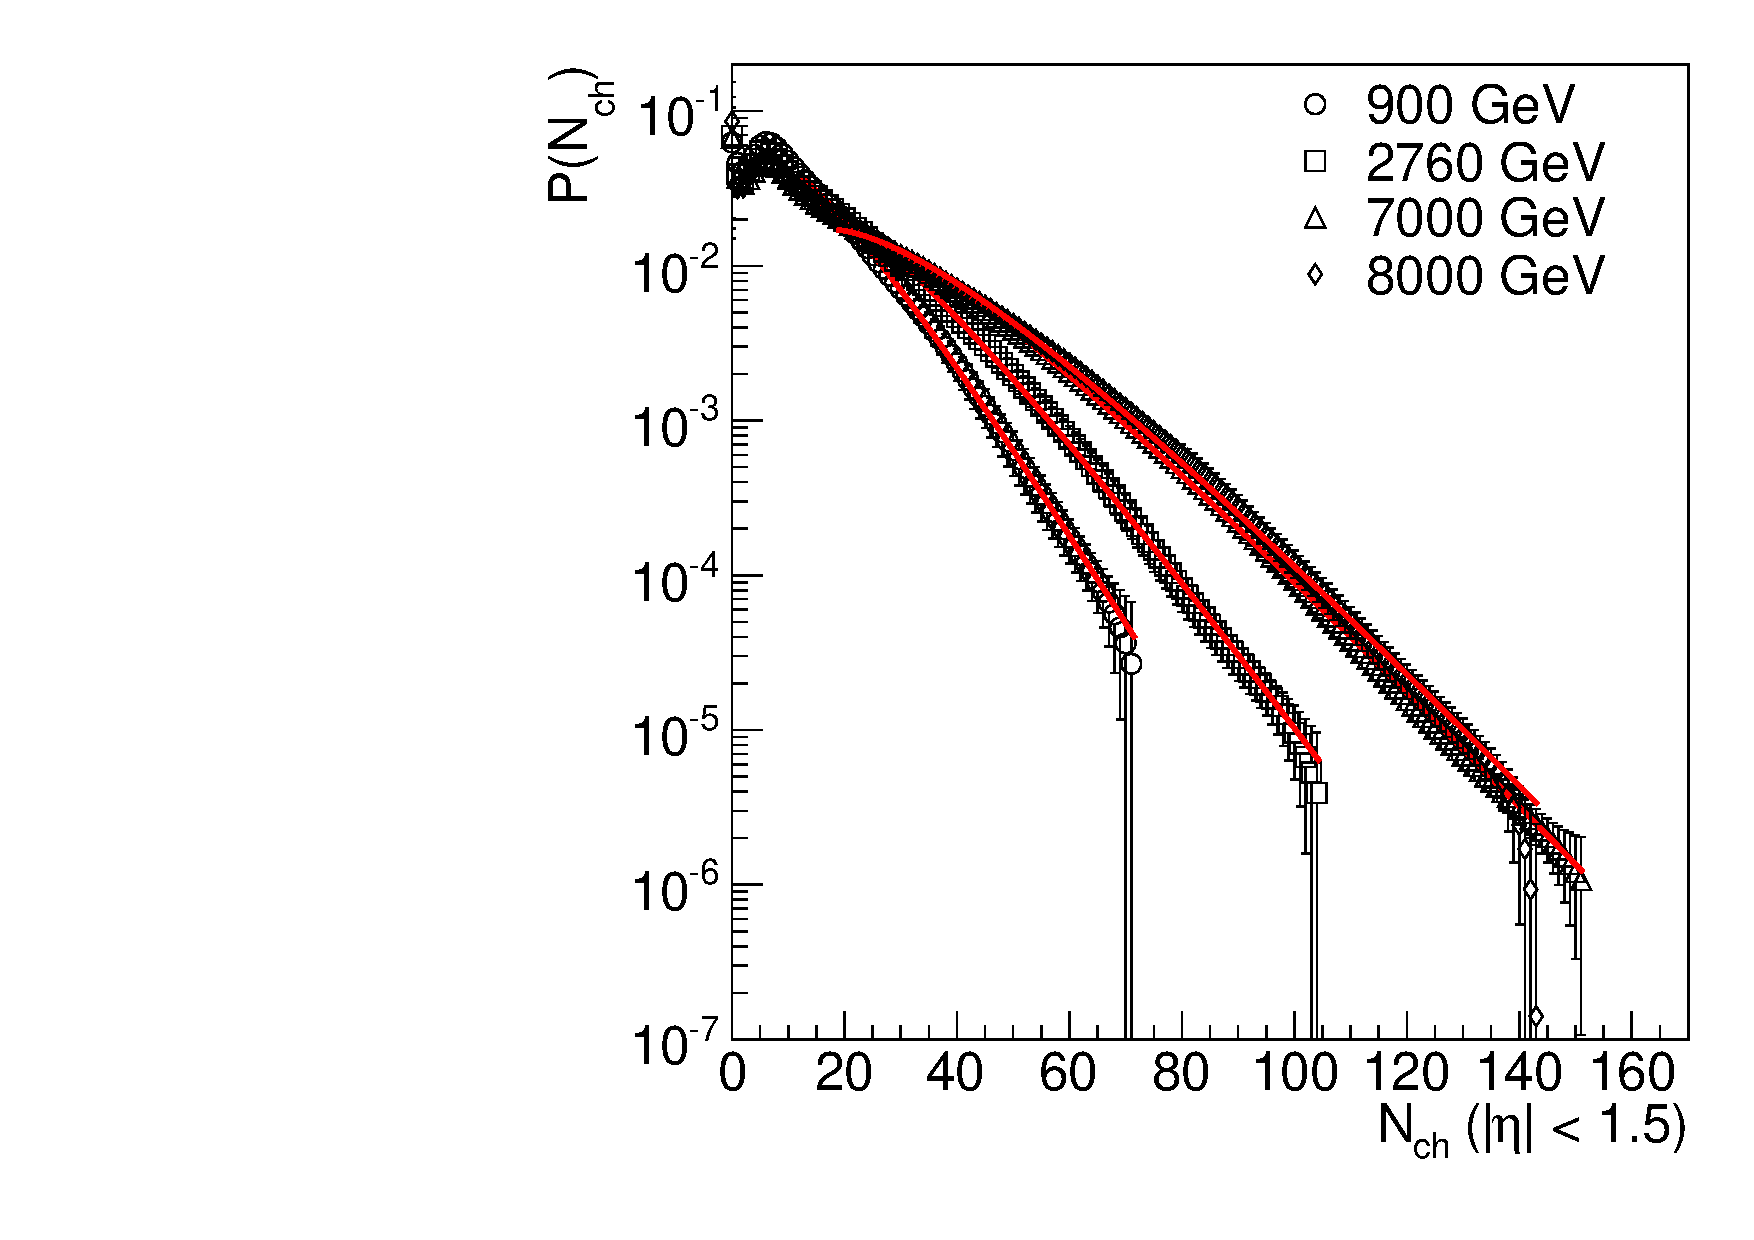
\includegraphics[width=0.49\linewidth]{\main/smallsystems/img/mult_data_1.pdf}
\hfill
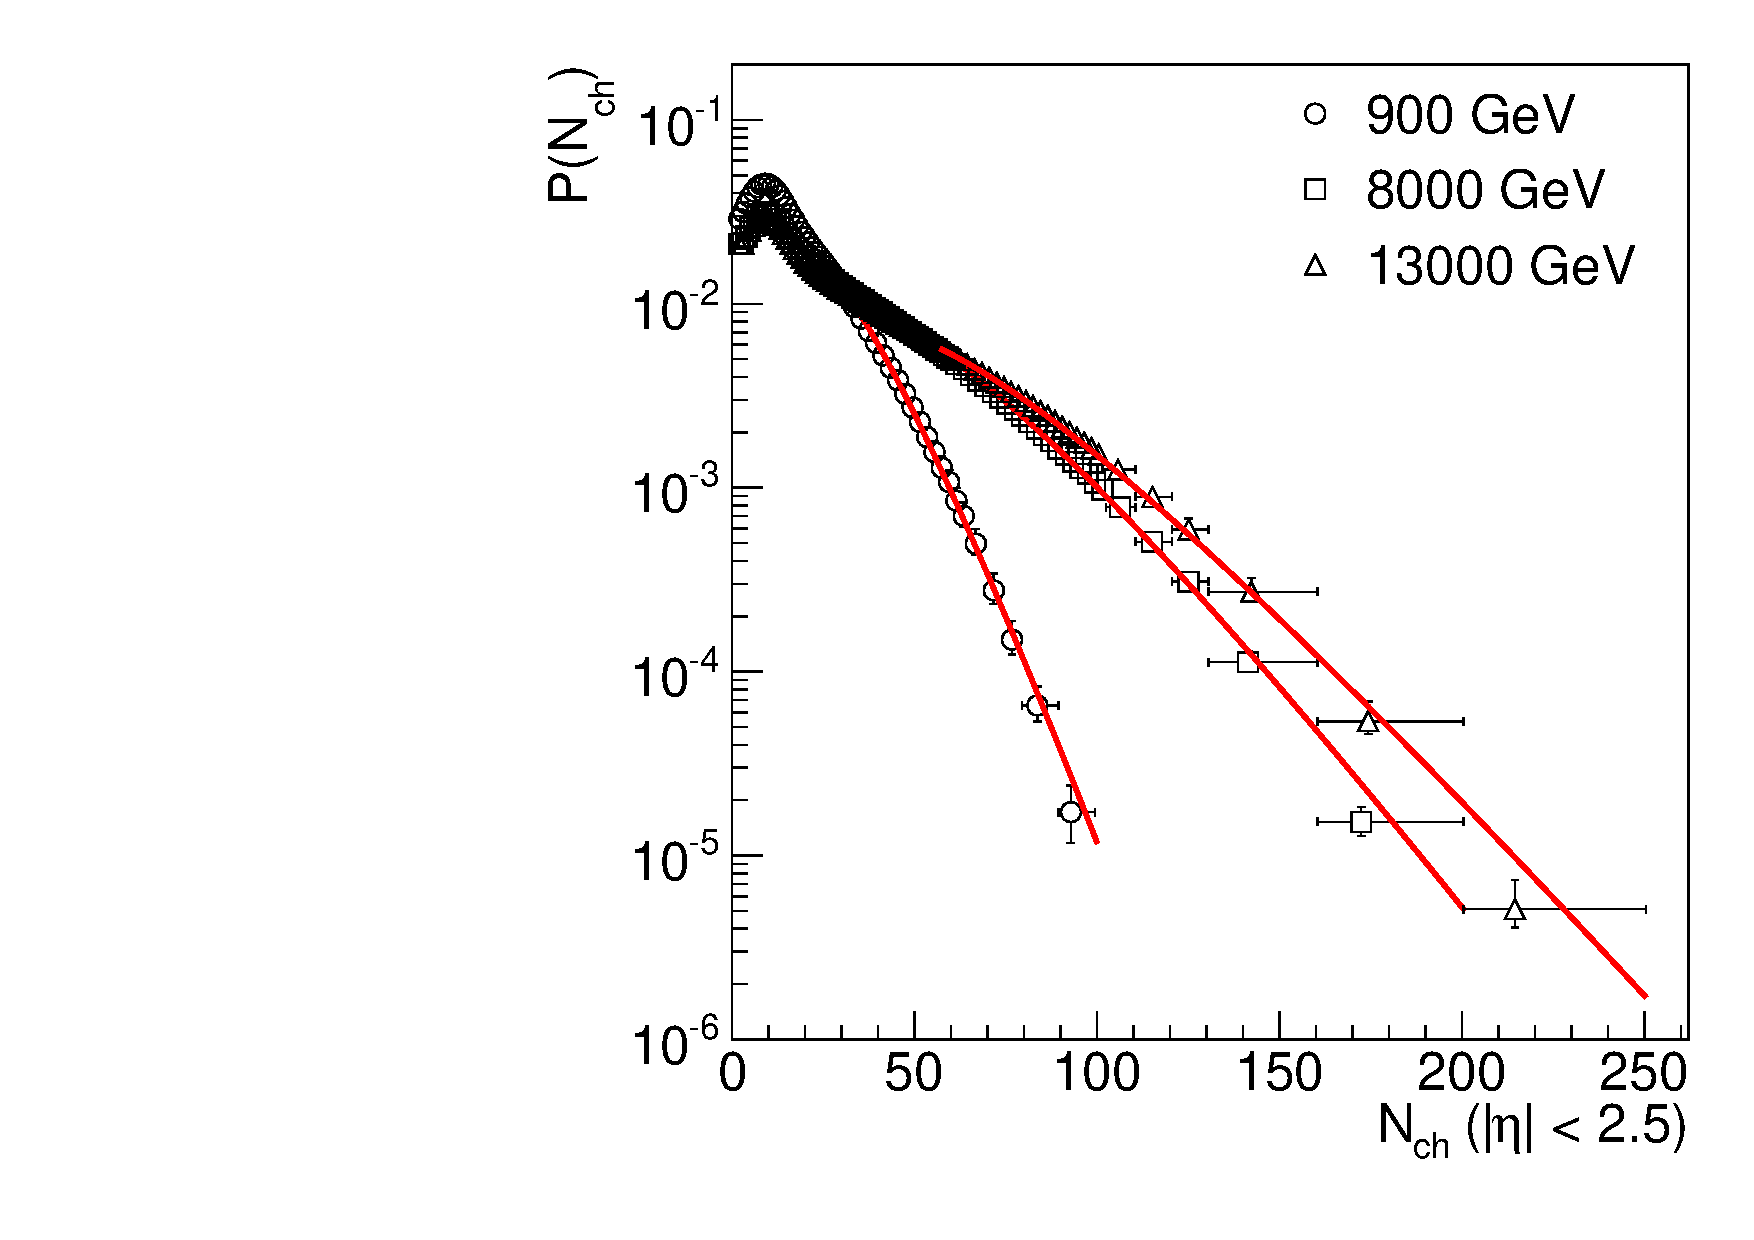
\includegraphics[width=0.49\linewidth]{\main/smallsystems/img/mult_data_11.pdf}
\caption{Multiplicity distributions measured by ALICE~\cite{Adam:2015gka} (left panel) and ATLAS\cite{Aad:2010ac,Aad:2016xww} (right panel) overlaid by the fit with a negative binomial distribution.}
\label{fig:smallsystems_mult_data}
\end{figure}

\begin{figure}[ht]
\centering
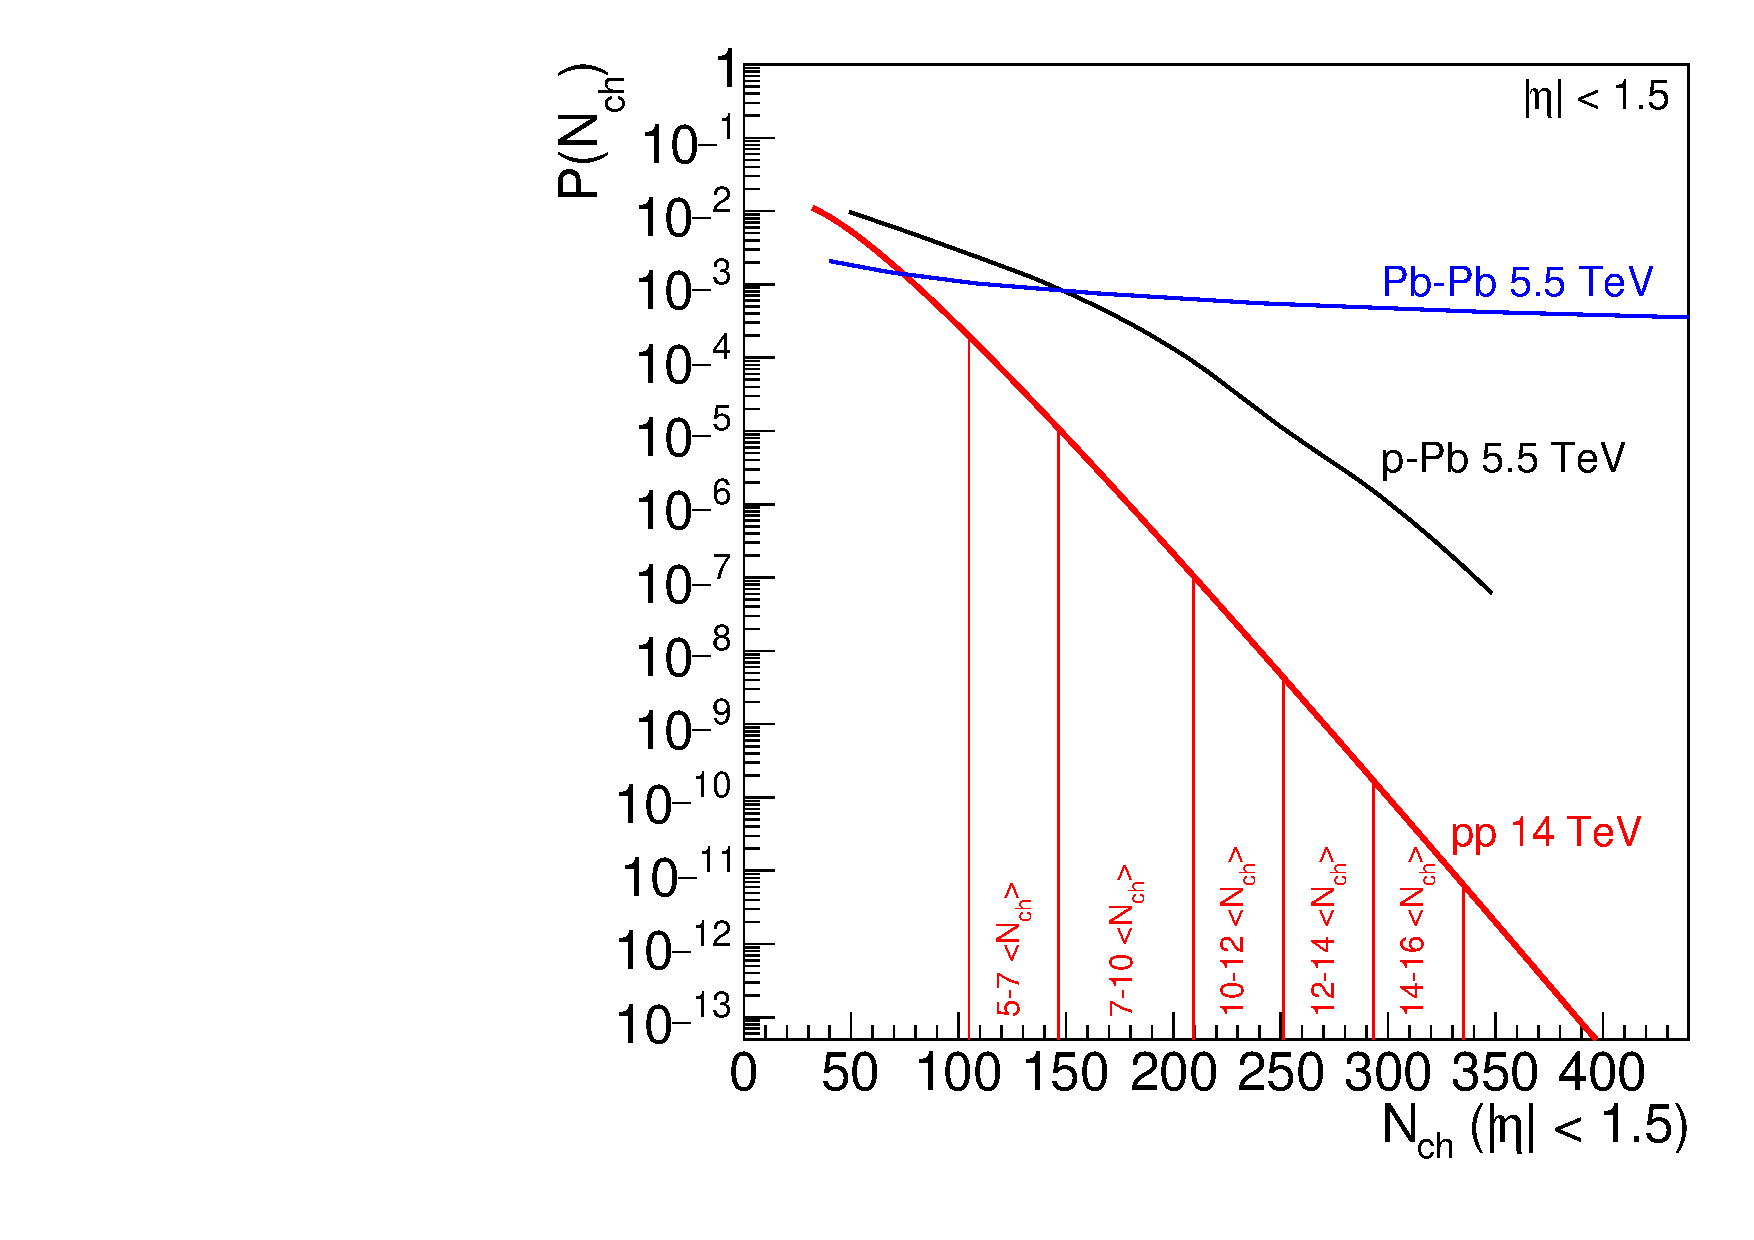
\includegraphics[width=0.32\linewidth]{\main/smallsystems/img/mult_extrapolation_alice.pdf}
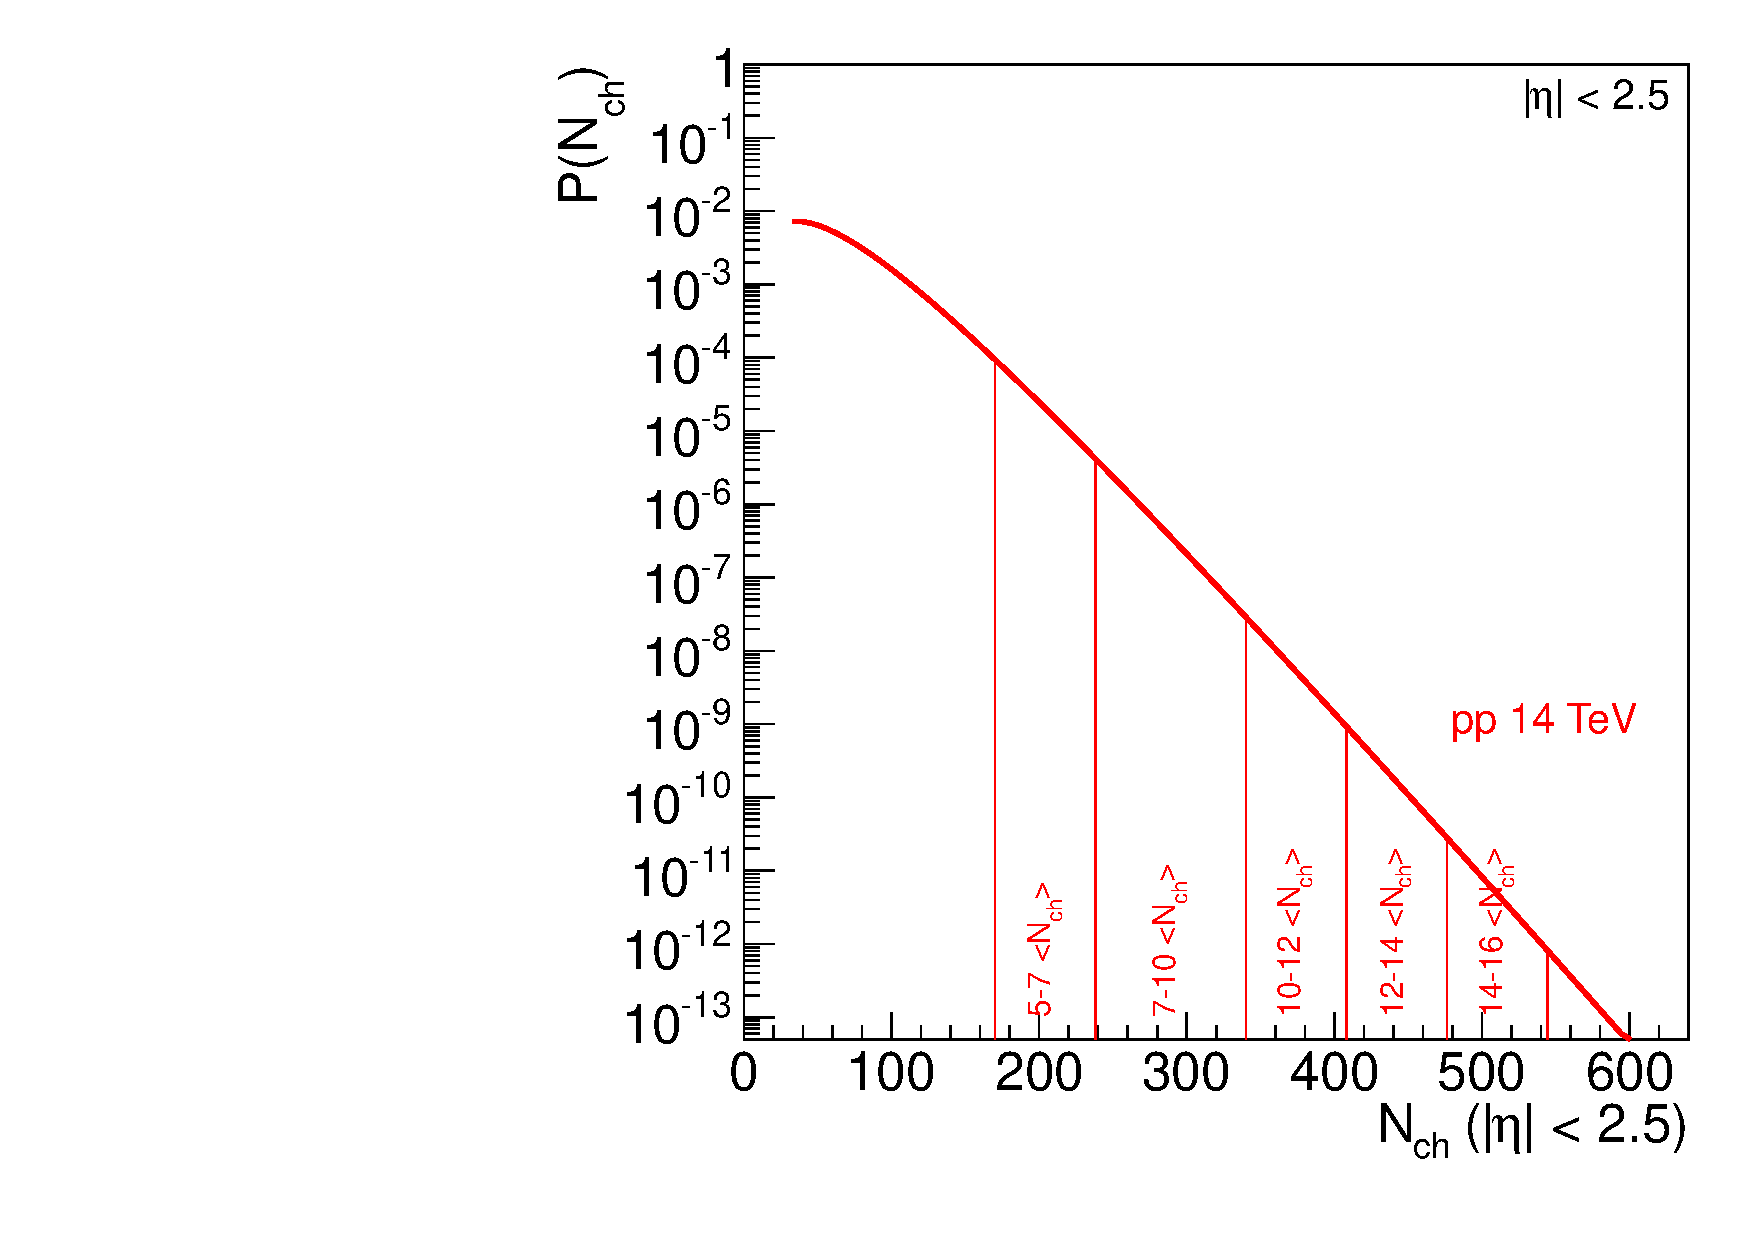
\includegraphics[width=0.32\linewidth]{\main/smallsystems/img/mult_extrapolation_atlas.pdf}
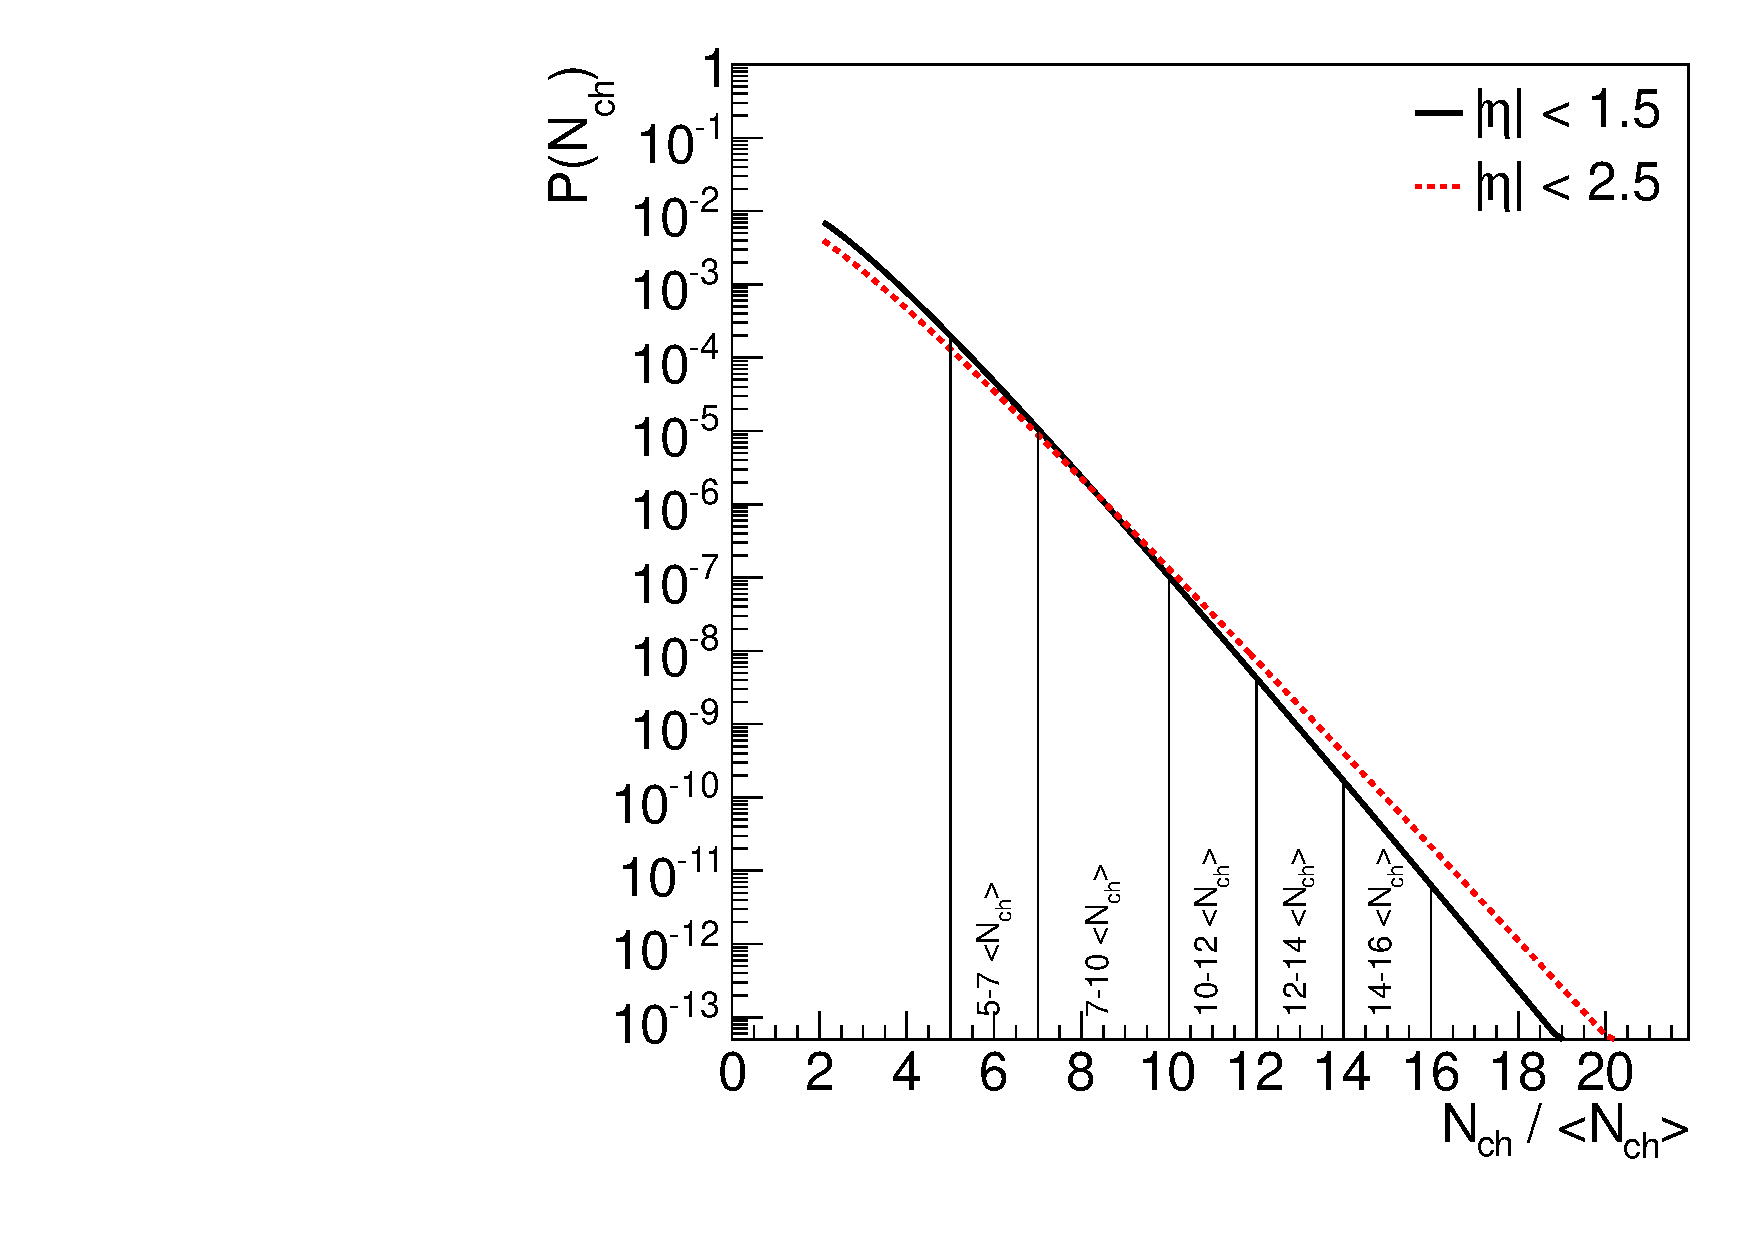
\includegraphics[width=0.32\linewidth]{\main/smallsystems/img/mult_extrapolation_comparison.pdf}
\caption{Extrapolated multiplicity distributions in pp collisions within $|\eta| < 1.5$ (left panel) and $|\eta| < 2.5$ (center panel). The indicated regions are from left to right for 5--7, 7--10, 10--12, 12--14, 14--16 times the average multiplicity. In the left panel the multiplicity distribution of \PbPb and \pPb collisions is also plotted. The right panel compares these two distributions scaled by the average multiplicity. The extrapolation for $|\eta| < 2.5$ turns out to be a bit wider at large multiplicities; therefore the one based on $|\eta| < 1.5$ is used as baseline.}
\label{fig:smallsystems_mult_extrapolation}
\end{figure}

The resulting extrapolated multiplicity distribution for 14~$\tev$ is shown in Fig.~\ref{fig:smallsystems_mult_extrapolation} for the ALICE and ATLAS case. In addition, these are compared scaled by their respective average multiplicities. The agreement is rather good, with some discrepancy in the tail of the distribution. The extrapolation based on the smaller phase space region falls off more quickly with multiplicity, and is therefore used as the more conservative estimate for all extrapolations.

\begin{figure}[ht]
\centering
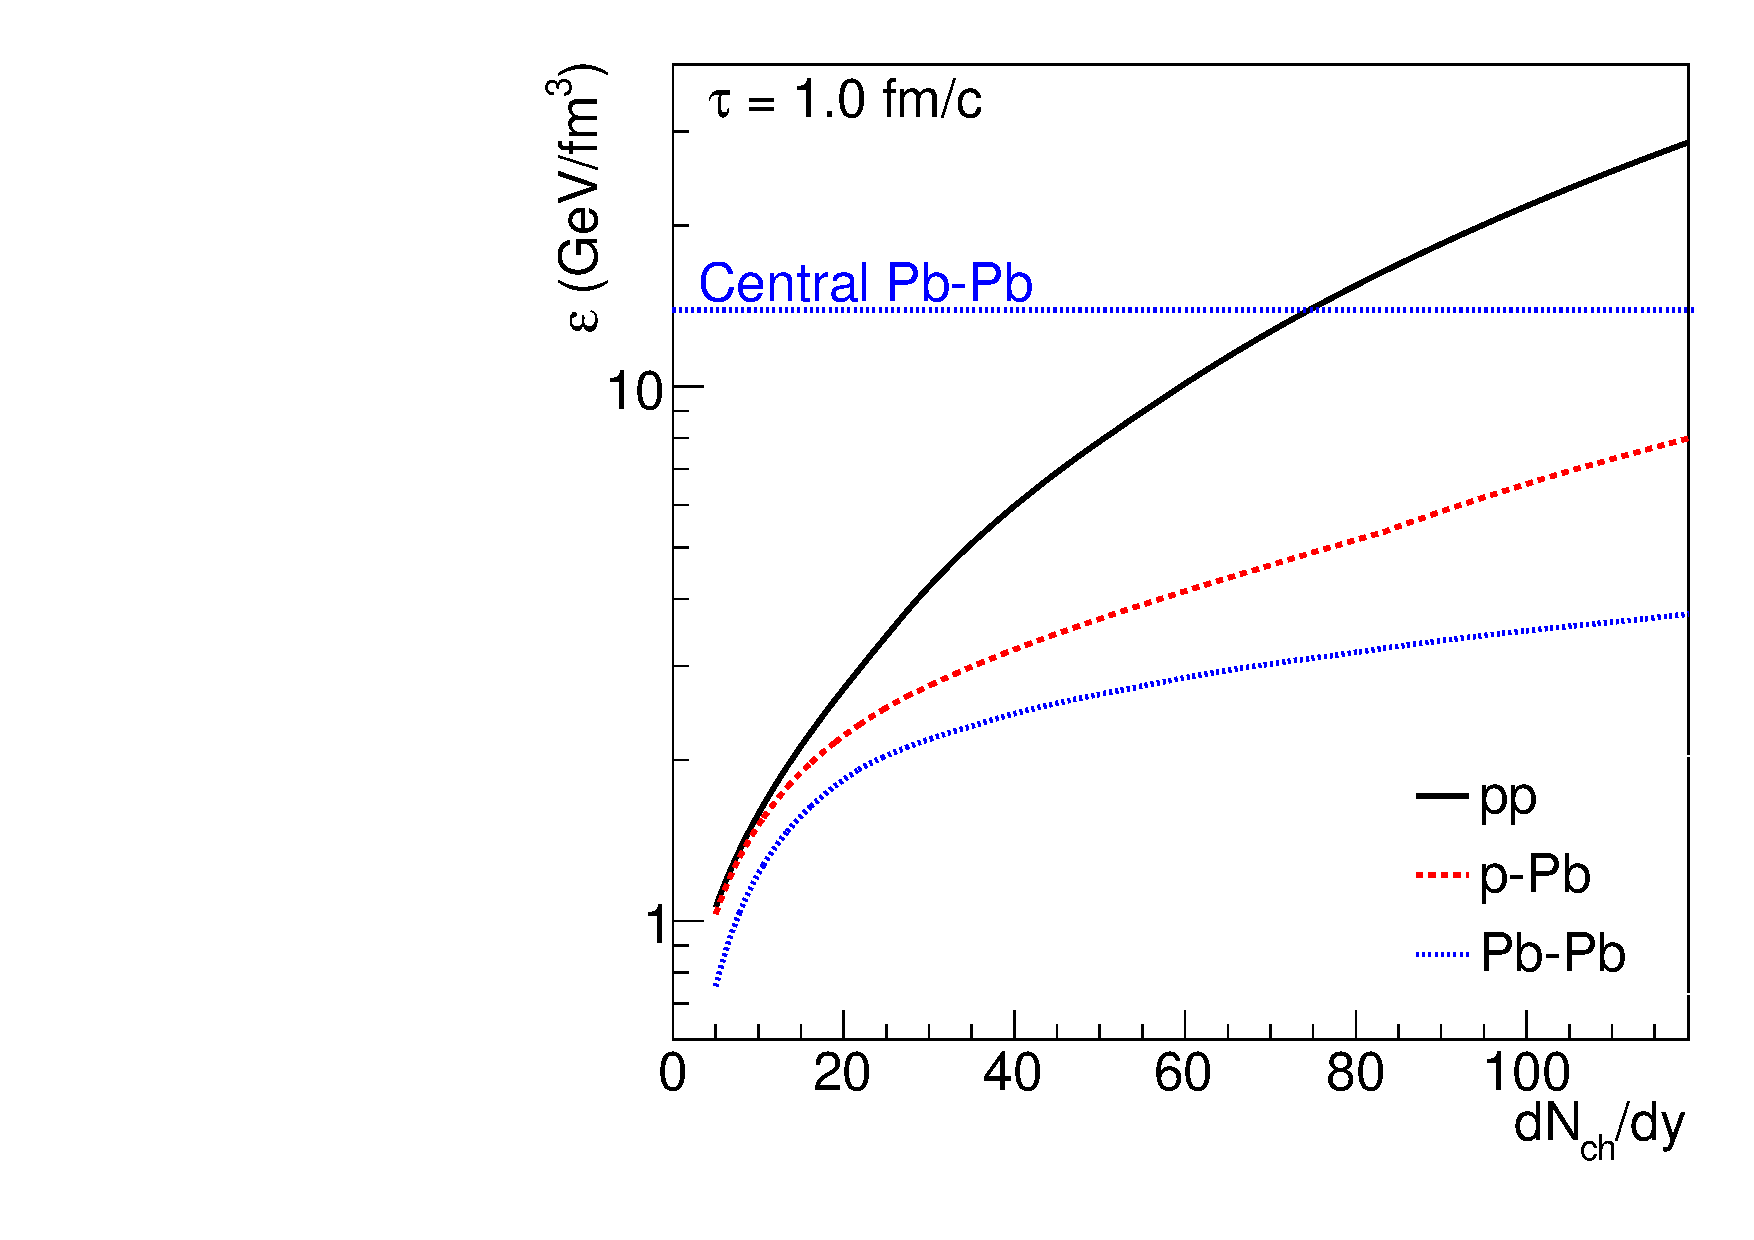
\includegraphics[width=0.5\linewidth]{\main/smallsystems/img/energy_density.pdf}
\caption{Energy density as a function of $\dNdy$ calculated by IP Glasma (solid lines) and with MC Glauber and the Bjorken formula (dashed lines); for details please see text. Compared are \pp, \pPb, and \PbPb at $\tau = \unit[0.2]{fm/c}$. The horizontal line indicates the energy density reached in central \PbPb collisions ($\dNdy \approx 2000$).}
\label{fig:energy_density}
\end{figure}

While the multiplicity is a convenient and well defined observable to compare different collision systems, the underlying dynamics may be driven by other properties. In large collision systems, the energy density $\epsilon$ is often used to characterize the system and the expected effects. Figure~\ref{fig:energy_density} shows an estimate of the energy density for \pp, \pPb and \PbPb collisions based on IP-Glasma~\cite{Bzdak:2013zma,SchenkePriv1} as well as on the Bjorken estimate:
\begin{equation}
  \epsilon = \frac{1}{A \tau} \langle E \rangle \frac{3}{2} \frac{dN_{ch}}{dy}.
\end{equation}
For the latter, the input is the multiplicity-dependent $\meanpT$~\cite{Abelev:2013bla,Acharya:2018njl} as well as the multiplicity-dependent transverse overlap from a Glauber MC~\cite{Loizides:2017ack}. The energy density is calculated at a fixed $\tau = \unit[0.2]{fm/c}$. It should be noted that these assumptions can be challenged and other ways to calculate $\epsilon$ are available. Here the aim is only to show that the energy density depends on the system at a fixed multiplicity, and can reach large values in \pp and \pPb collisions, of the order of central \PbPb collisions.

Table~\ref{tab:smallsystems_pp} gives the fraction of cross-section and the number of events in 5 multiplicity classes:  5--7, 7--10, 10--12, 12--14 and 14--16 times the average multiplicity. Table~\ref{tab:smallsystems_pbpb} gives the number of events of bins with equivalent multiplicity than commonly measured multiplicity bins in \pPb and \PbPb collisions. For the calculation of the number of events $\sigma_{\rm inel} = \unit[78.4]{mb}$~\cite{Loizides:2017ack} is used. These tables are the key input for the performance figures presented in this section. A high-multiplicity \pp program sampling \unit[200]{pb$^{-1}$} is assumed for all experiments. 
The conversion of the provided $\dNdeta$ to multiplicity ranges with larger pseudorapidity coverage is done for simplicity assuming a flat pseudorapidity distribution within $|\eta| < 2.5$. For the conversion with $\pT$ cuts as employed in many current measurements a set of conversation factors is used, listed in Tab.~\ref{tab:smallsystems_conversion}.
 
\begin{table}
\centering
\begin{tabular}{c|c|c|c|c}
Range & $\dNdeta$ & Fraction & Events per pb$^{-1}$ & Events in 200~pb$^{-1}$ \\
\hline
5--7 \meannch     & 35--49   & 2.4e-03       & 1.9e+08       & 3.7e+10 \\
7--10 \meannch    & 49--70   & 1.3e-04       & 1.0e+07       & 2.0e+09 \\
10--12 \meannch   & 70--84   & 1.1e-06       & 9.0e+04       & 1.8e+07 \\
12--14 \meannch   & 84--98   & 4.7e-08       & 3.7e+03       & 7.3e+05 \\
14--16 \meannch   & 98--112  & 1.8e-09       & 1.4e+02       & 2.8e+04 \\
\hline
\end{tabular}
\caption{Number of pp events at 14 $\tev$ in selected multiplicity bins.}
\label{tab:smallsystems_pp}
\end{table}

\begin{table}
\centering
\begin{tabular}{l|c|c|c}
Range & $\dNdeta$ & Events per pb$^{-1}$ & Events in 200~pb$^{-1}$ \\
\hline
0--5\% p--Pb   & 41--56        & 4.9e+07       & 9.8e+09 \\
5--10\% p--Pb  & 34--41        & 1.9e+08       & 3.8e+10 \\
10--20\% p--Pb & 27--34        & 6.6e+08       & 1.3e+11 \\
\hline
60--65\% Pb--Pb    & 98--137       & 1.5e+02       & 3.0e+04 \\
65--70\% Pb--Pb    & 68--98        & 1.6e+05       & 3.1e+07 \\ 
70--75\% Pb--Pb    & 45--68        & 2.1e+07       & 4.2e+09 \\
75--80\% Pb--Pb    & 29--45        & 5.9e+08       & 1.2e+11 \\
\hline
\end{tabular}
\caption{Number of events in pp collisions at 14 $\tev$ sliced in equivalent multiplicity bins as in \pPb and \PbPb collisions.}
\label{tab:smallsystems_pbpb}
\end{table}

\begin{table}
\centering
\begin{tabular}{c|c|c|c|c|c}
\backslashbox{$|\eta|$}{$\pT$} & $> \unit[0.1]{\UGeVc}$ & $> \unit[0.2]{\UGeVc}$ & $> \unit[0.3]{\UGeVc}$ & $> \unit[0.4]{\UGeVc}$ & $> \unit[0.5]{\UGeVc}$ \\
\hline
$|\eta| < 1.5$ & 1.03 & 1.11 & 1.22 & 1.31 & 1.40 \\
\hline
$|\eta| < 2.4$ & 1.04 & 1.14 & 1.27 & 1.42 & 1.55 \\
\hline
\end{tabular}
\caption{Conversion factors between $\nch$ with a $\pT$ threshold, and $\nch$ including particles down to $\pT = 0$. The factor shown is $\nch / \nch(\pT > X)$, extracted with Pythia 8, tune CUETP8M1. A potential multiplicity dependence of this factor is neglected for the projections in this document.}
\label{tab:smallsystems_conversion}
\end{table}

\subsubsection{Global-Event Properties}

The measurement of global-event observables in rare high-multiplicity \pp collisions are of interest in itself. The shape of the multiplicity distribution, which has been largely extrapolated in the previous section, is today a challenge for models. It is not clear which mechanisms produce very large multiplicity events and therefore the shape of the distribution is an important input. Studies of $\meanpT$ as a function of multiplicity~\cite{Abelev:2013bla} have shown a strong increase with multiplicity. However, those measurements exist only up to $\dNdeta \approx 55$, while the measurements at HL-LHC promise a measurement beyond twice that value. High-multiplicity collisions are understood as originating from the collision of multiple partons within the same \pp collisions. It has been shown that the number of (low $Q^2$) parton interactions increase linearly with multiplicity with a hint of a saturation at large multiplicity~\cite{Abelev:2013sqa}. A continuation of this study at higher multiplicity with the prospect of showing that there is a maximal number of parton interactions is an important ingredient to a better understanding of particle production in high-energy pp collisions.

\subsubsection{Particle Correlations}

The measurements of two-particle correlations and higher-order cumulants have produced the initial observations of collective-like effects in small systems. In \pp collisions, two distinct regions are of interest at HL-LHC: the high-multiplicity tail to compare to \pPb and \PbPb collisions and the low-multiplicity regions to see the onset of these effects. In the following, several performance estimates are given as examples for the rich physics which can be addressed. 

State-of-the-art measured 4-particle cumulants of $v_3$ ($c_3\{4\}$) in \pp and \pPb collisions are presented in Fig.~\ref{fig:smallsystems_corr_cumulants} overlaid with the projection for HL-LHC. 
In order to remove non-flow contributions, the 3-subevent method is applied. In \pp collisions, with the data collected in Run 2, the statistical uncertainties are large and the $c_3\{4\}$ values are systematically consistent with zero in most of the $\nch$ range. On the contrary, in large systems, significant non-zero $c_3\{4\}$ has been measured\todo{give values and REF for \PbPb measurement in similar \pT range, need to choose a centrality interval or give range.}, which reflects the nucleonic fluctuations in the initial state. Whether similar behavior is observed in small systems still needs to be confirmed. The increase in luminosity in Run 3 and Run 4 provides a great opportunity to measure $c_3\{4\}$ in pp with high precision: the statistics are sufficient to measure a signal as small as $v_3\{4\} = 1.5\%$ for $\nch \gtrapprox 170$, while 2\% are accessible with large significance over a wide multiplicity range ($\nch \gtrapprox 100$). Similarly, in \pPb collision, the current result shows that $c_3\{4\}$ is consistent with zero, but increased statistics will help to detect a potential non-zero $c_3\{4\}$ smaller than $1.5\%$ for $100 \lessapprox \nch \lessapprox 500$. Similarly, the precision of the already measured non-zero $c_2\{4\}$ will be greatly improved\todo{can we refer to a CONF note?}.

\begin{figure}[ht]
\centering
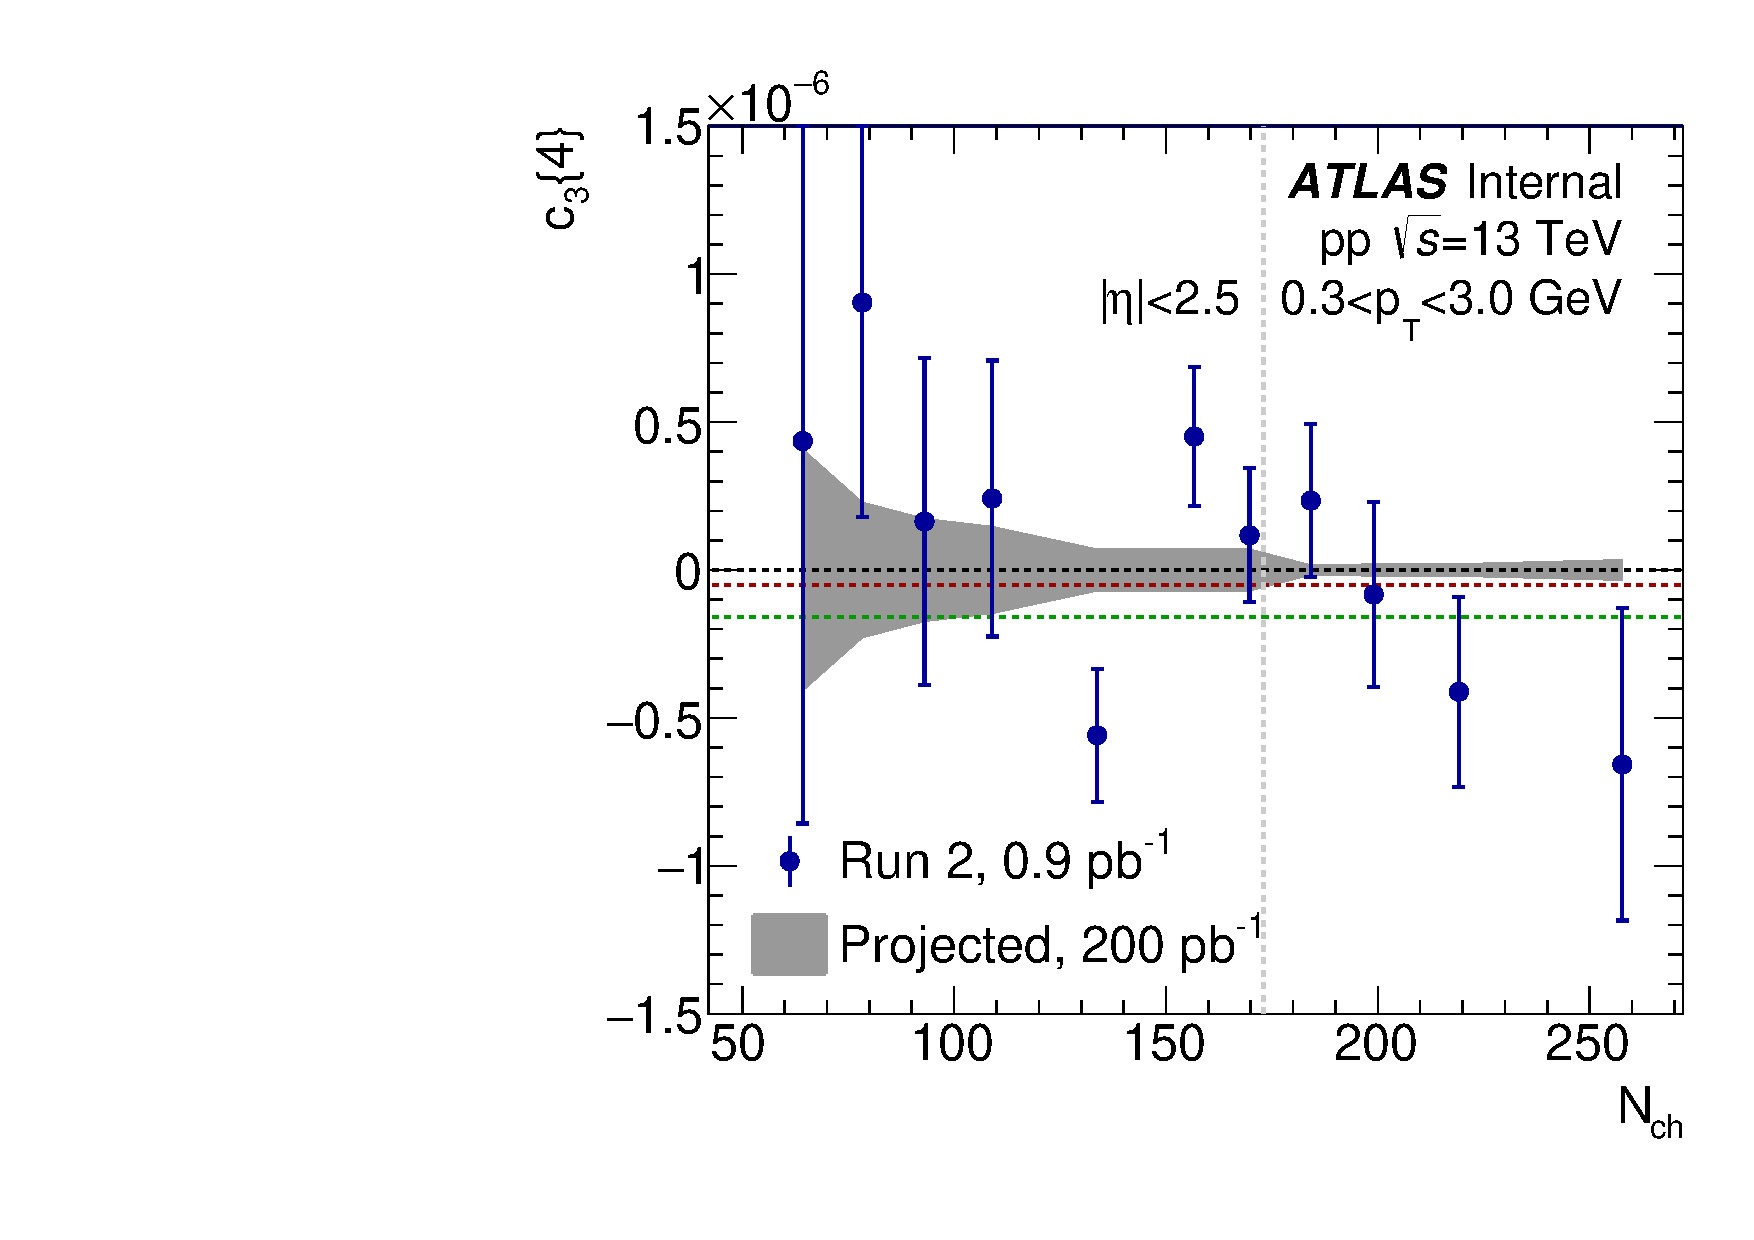
\includegraphics[width=.49\linewidth]{\main/smallsystems/img/c_3_4_pp.pdf}
\hfill
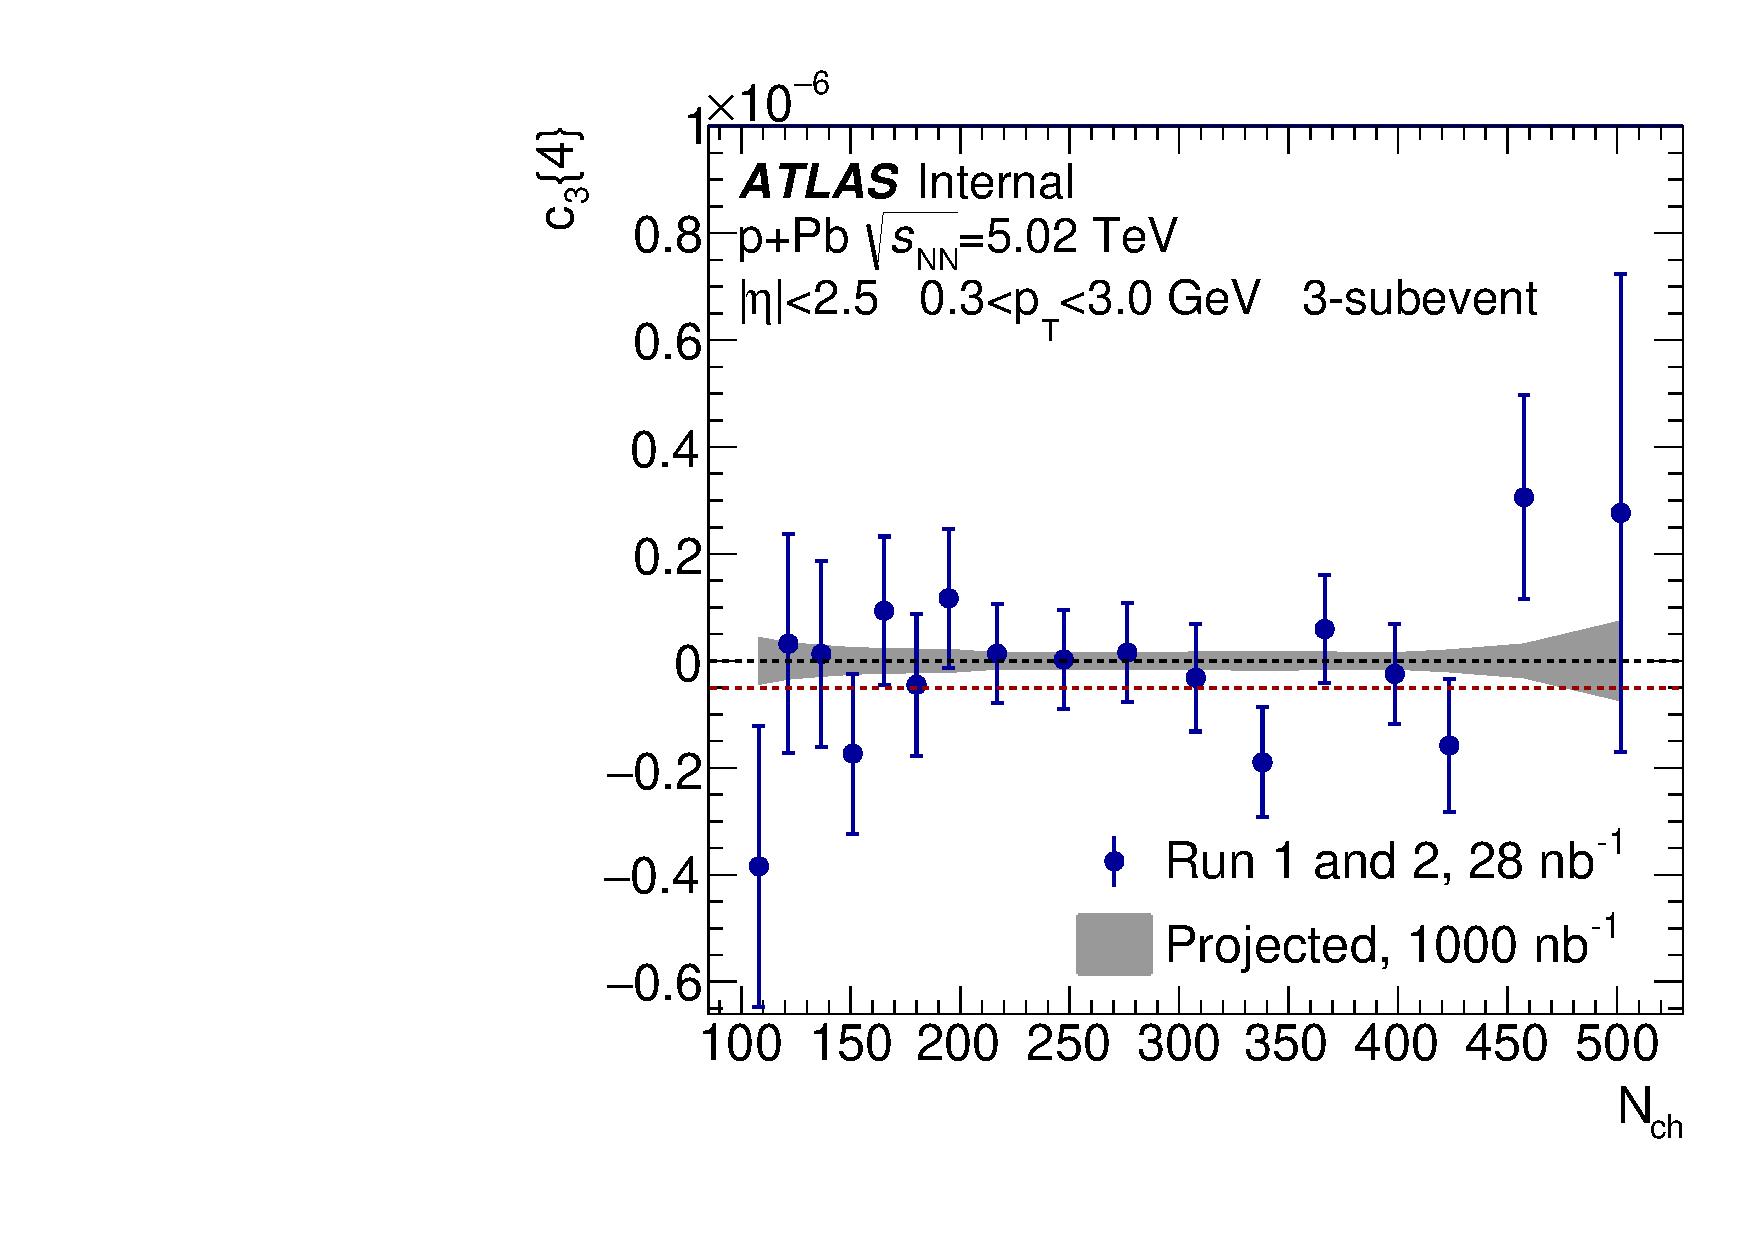
\includegraphics[width=.49\linewidth]{\main/smallsystems/img/c_3_4_pPb.pdf}
\caption{4-particle cumulants $c_3\{4\}$ with 3-subevent method for \pp (left) and \pPb (right) as a function of $\nch$. Only statistical uncertainties are shown in the figure and the gray band represents the projected statistical uncertainty, with $c_3\{4\}$ assumed to be zero. The red and green dash lines represent $1.5\%$ and $2.0\%$ $v_3\{4\}$ signal respectively. The horizontal line in the left panel indicates the the transition between minimum-bias data and high-multiplicity triggered data. Figure from Ref.~\cite{}.}
\label{fig:smallsystems_corr_cumulants}
\end{figure}

\begin{figure}[ht]
\centering
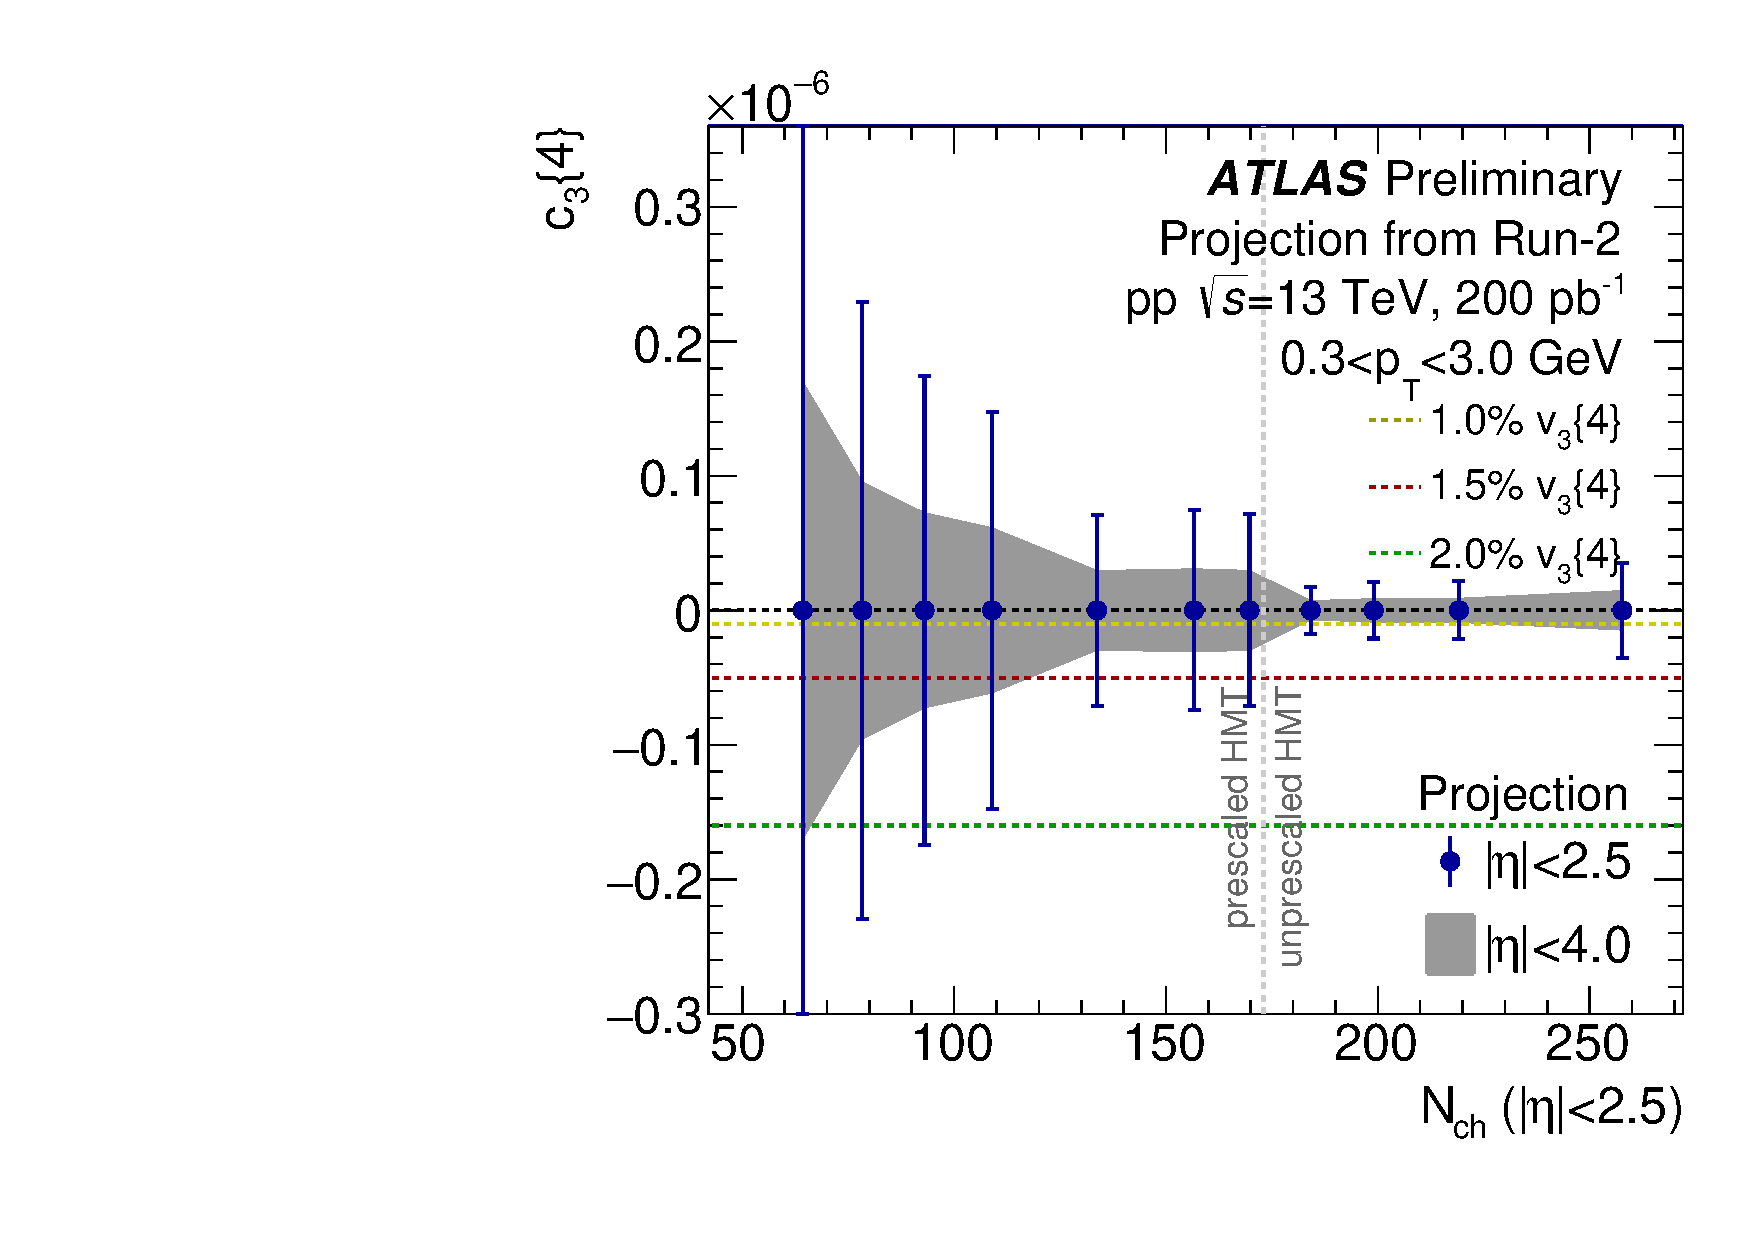
\includegraphics[width=.49\linewidth]{\main/smallsystems/img/c_3_4_pp_eta4.pdf}
\caption{Demonstration of the influence of the larger tracking acceptances for ATLAS and CMS available in Run 4. The figure shows the 4-particle cumulants $c_3\{4\}$ as in Fig.~\ref{fig:smallsystems_corr_cumulants} for \pp collisions with $\Lint = \unit[200]{pb^{-1}}$. The data points indicate the reach with the current detector ($|\eta| < 2.5$) while the gray band the enlarged acceptance of $|\eta| < 4$.}
\label{fig:smallsystems_corr_cumulants_eta4}
\end{figure}




% \begin{figure}[ht]
% \centering
% 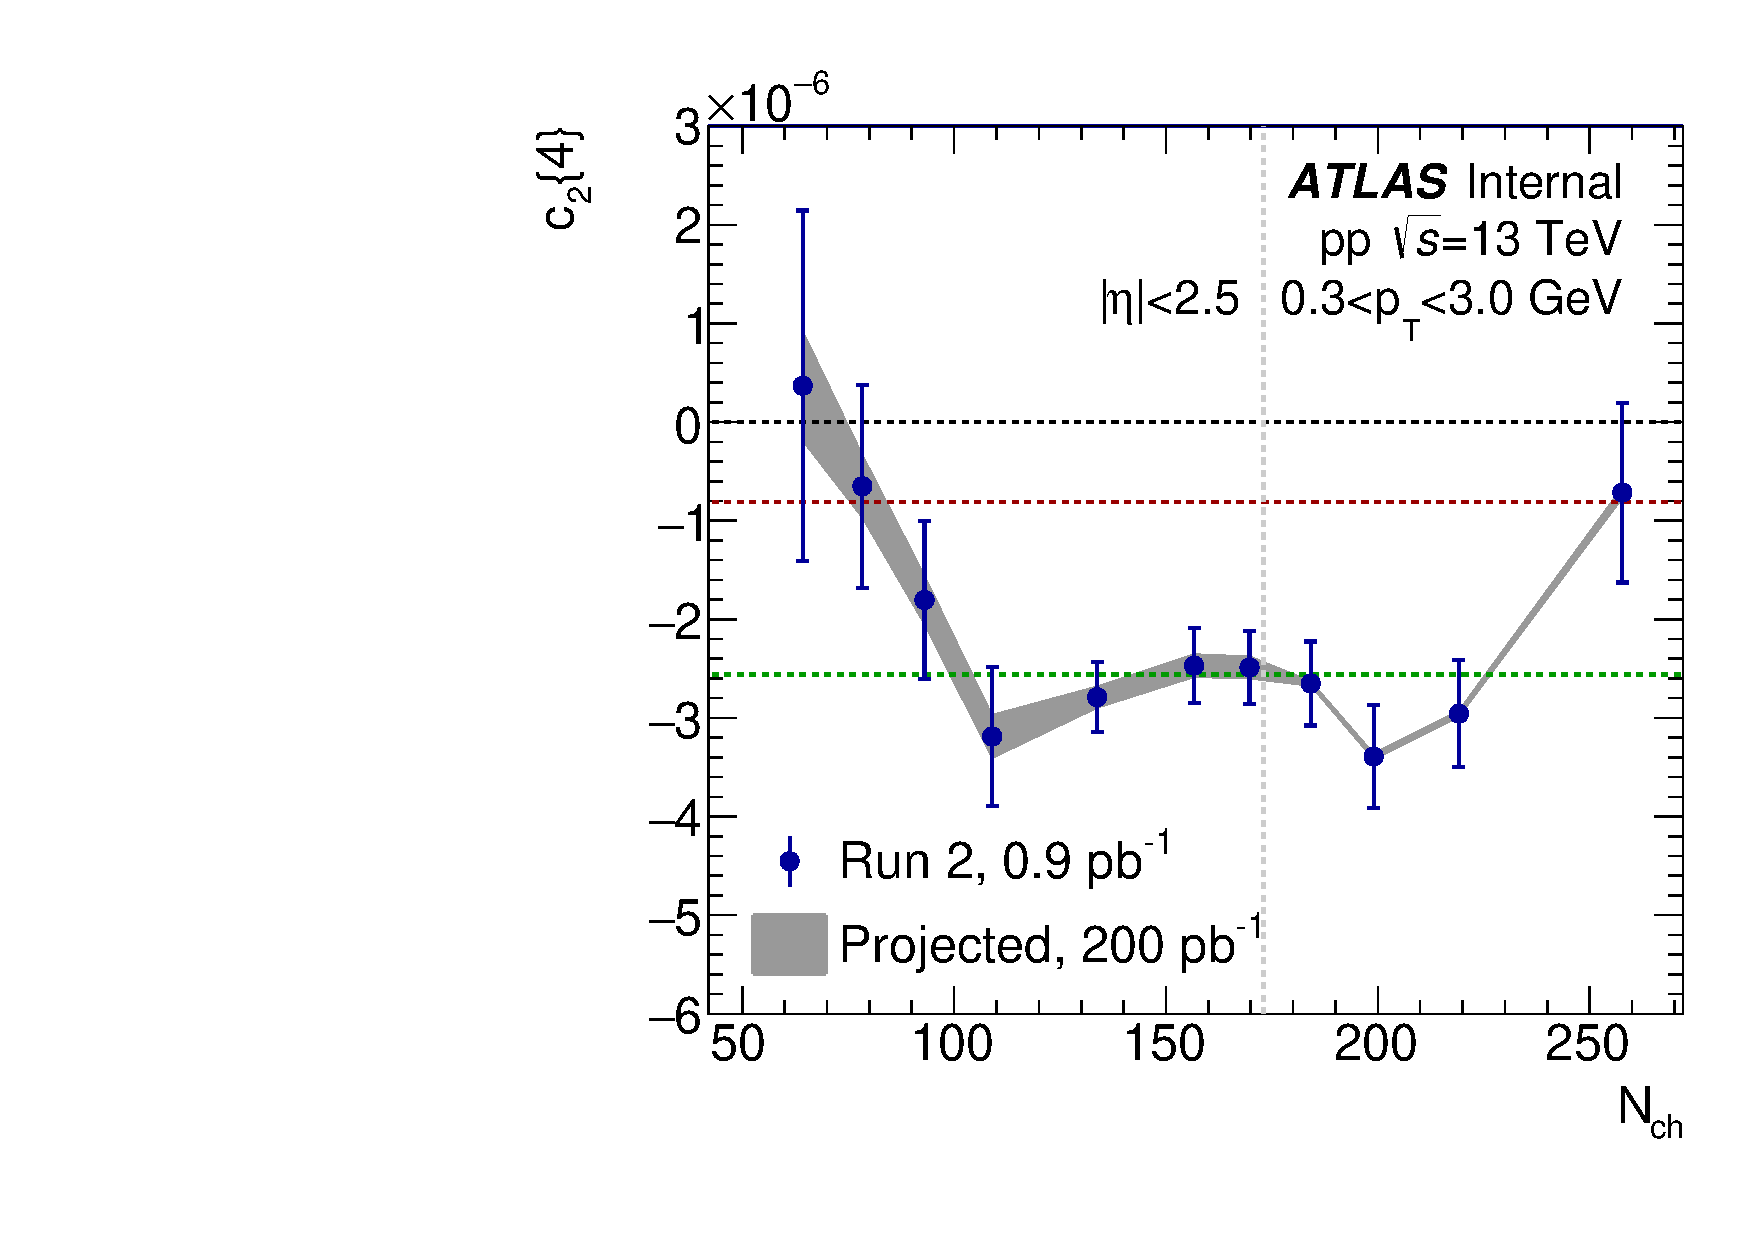
\includegraphics[width=.45\linewidth]{\main/smallsystems/img/c_2_4_pp.pdf}
% 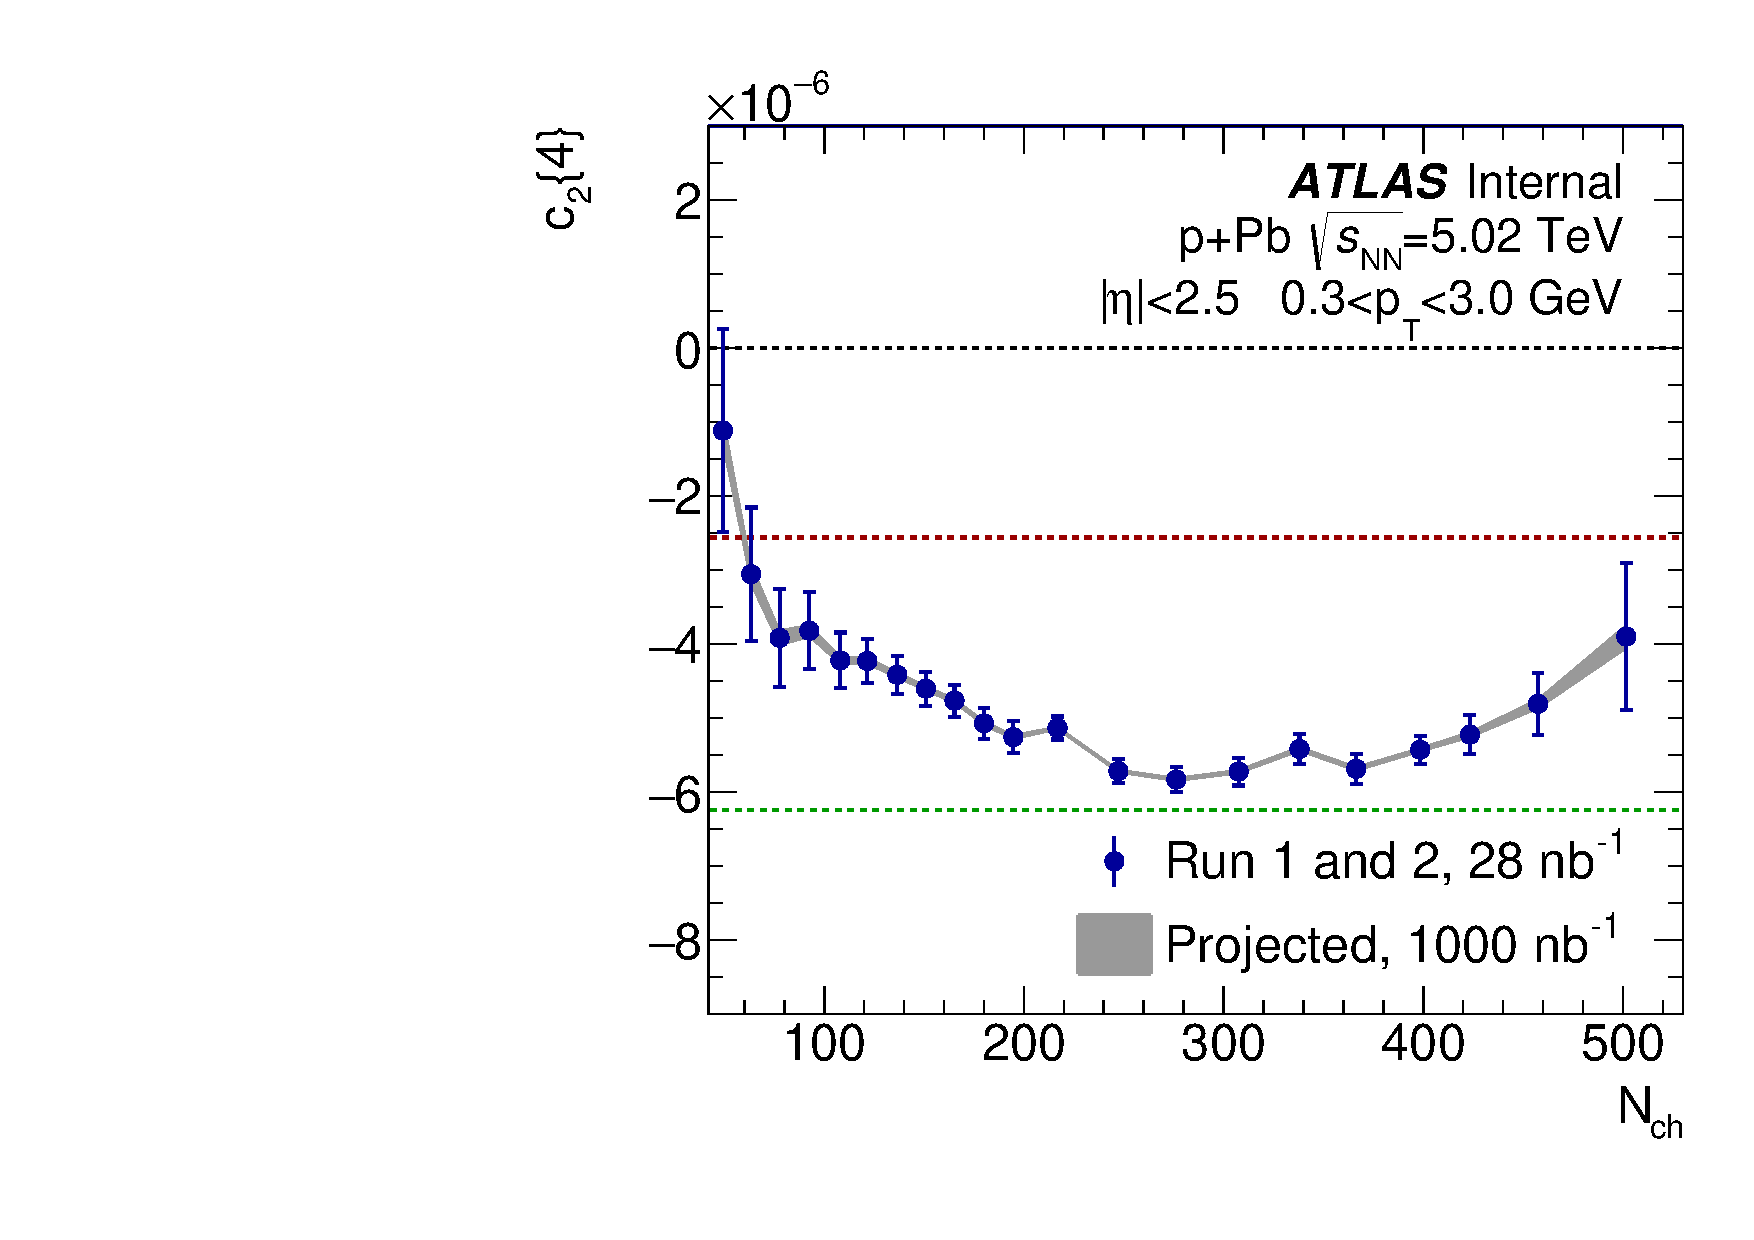
\includegraphics[width=.45\linewidth]{\main/smallsystems/img/c_2_4_pPb.pdf}
% \caption{4-particle cumulants $c_2\{4\}$ with 3-subevent method for $pp$ (left) and $p$+Pb (right) as a function of $N_{ch}$. Only statistical uncertainties are shown in the figure and the gray band represents the projected statistical uncertainty. The red and green dash lines represent $3\%$ and $4\%$ $v_2\{4\}$ signals for $pp$, and $4\%$ and $5\%$ $v_2\{4\}$ signals for $p$+Pb. The horizontal line in the left panel indicates the the transition between minimum-bias data and high-multiplicity triggered data. Figure from Ref.~\cite{}. {\bf Figure to be removed, only to be discussed in the text.}}
% \label{fig:smallsystems_corr_cumulants_v2}
% \end{figure}

The correlations of flow harmonics between different orders, called symmetric cumulants, are very sensitive to the initial state and the hydrodynamic evolution. In \PbPb collisions these are, for instance, used to constrain the shear viscosity over entropy ratio $\eta/s$. In addition, they challenge the description of the observed phenomena within initial state saturation models.
Their measurement in small systems can provide important insight in the validity of the hydrodynamic description of the observed phenomena. The present uncertainties of such measurement in small systems are too large for a definitive conclusion, in particular in \pp collisions, due to the dominance of non flow like jets and resonance decays. Figure~\ref{fig:smallsystems_corr_symmetriccumulants} shows the performance projection of ${\rm SC}(2,3) = \langle v_2^2 v_3^2 \rangle - \langle v_2^2 \rangle \langle v_3^2 \rangle$ for HL-LHC for \pp and \pPb collisions. The uncertainties of the measurement without subevents becomes practically invisible, however, those stay dominated by non-flow effects. A measurement requiring two, three and even four subevents becomes possible with uncertainties of the order of few times $10^{-7}$ depending on multiplicity. Such results can give a definitive answer if a similar hydrodynamic footprint is observed in small and large systems.

\begin{figure}[t]
\centering
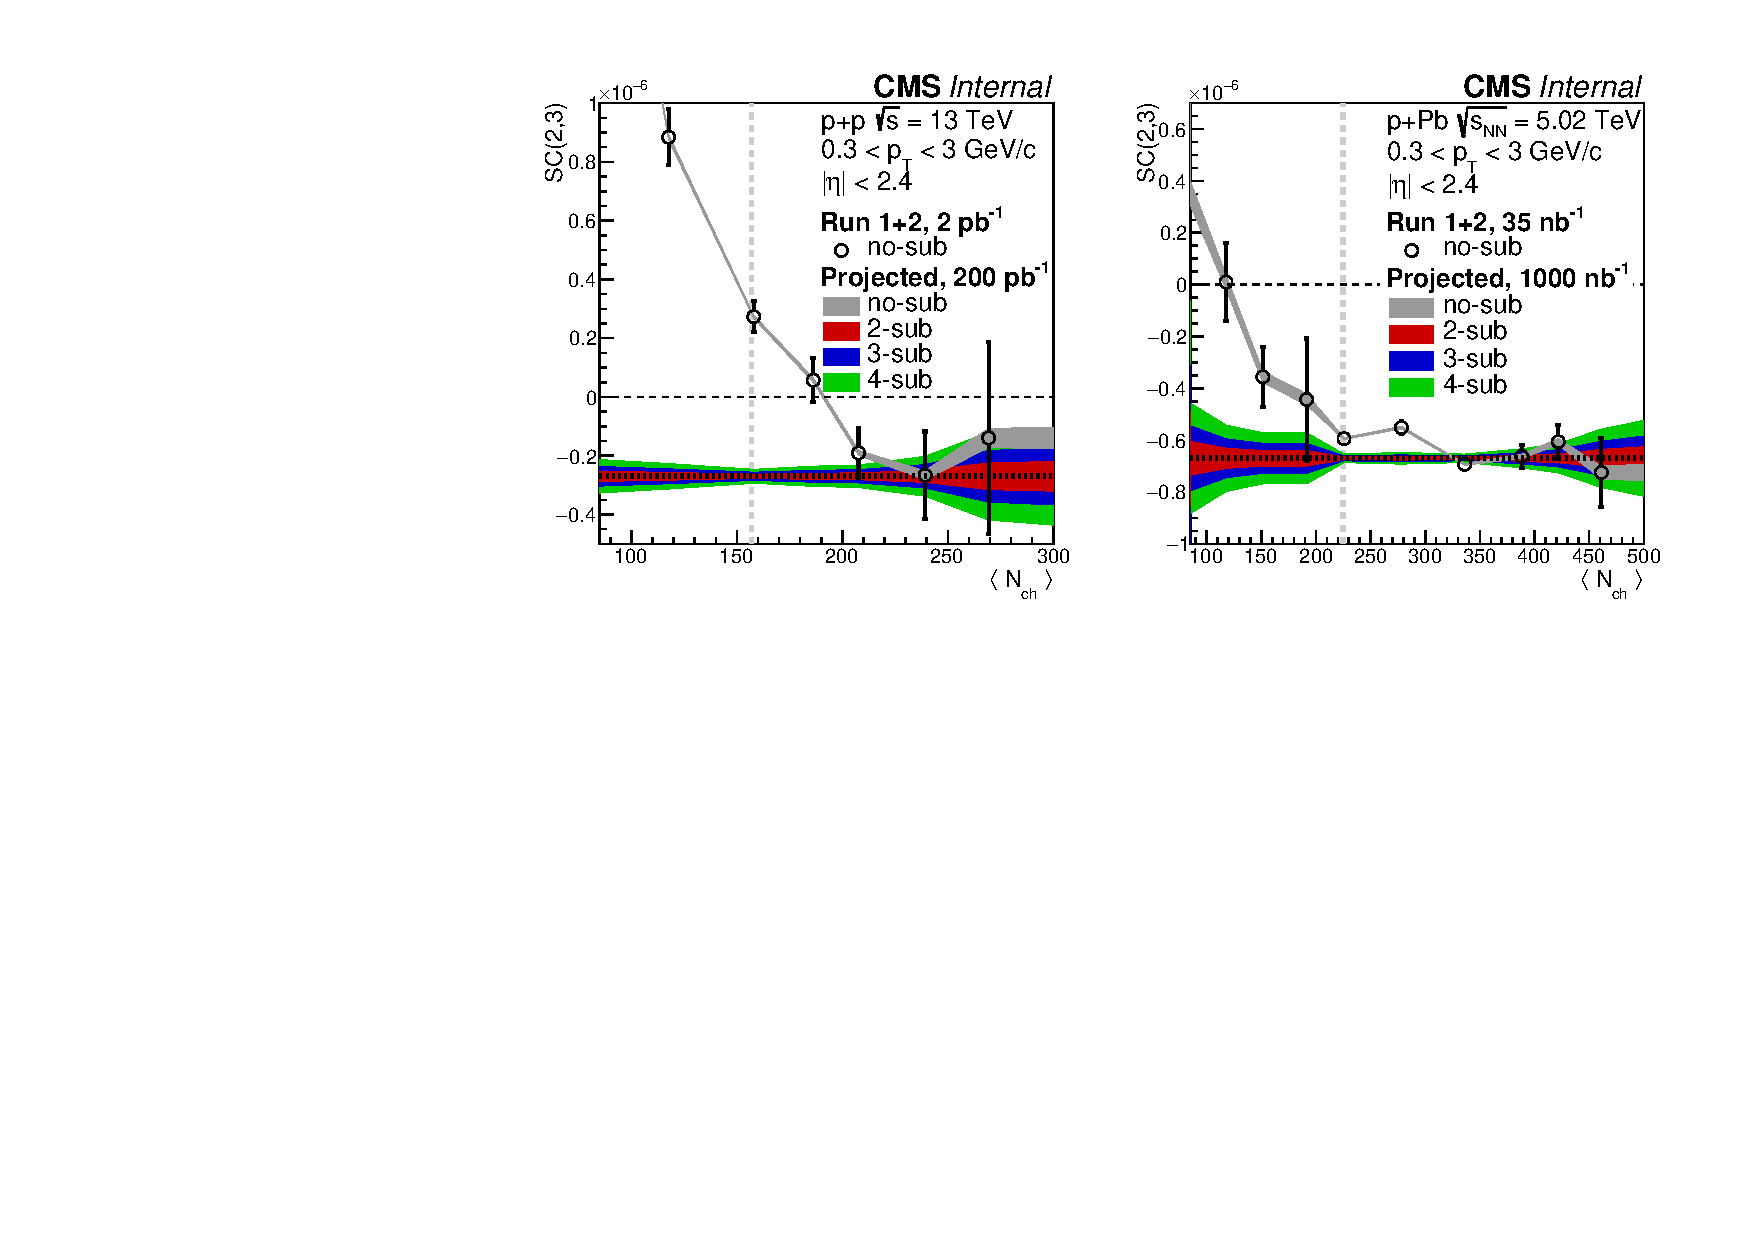
\includegraphics[width=\linewidth]{\main/smallsystems/img/HLLHC_SC.pdf}
\caption{Symmetric cumulants extracted with and without applying subevents for \pp (left) and \pPb (right) as a function of $\nch$. The projected reach is shown for the case of 2, 3 and 4 subevents assuming a constant signal as a function of multiplicity indicated by the lower horizontal line. The vertical line indicates the transition between minimum-bias data and high-multiplicity triggered data. Figure from Ref.~\cite{}.}
\label{fig:smallsystems_corr_symmetriccumulants}
\end{figure}

Figure~\ref{fig:smallsystems_corr_cumulants_pid}

\begin{figure}[ht]
\centering
\includegraphics[width=.49\linewidth,draft]{\main/smallsystems/img/v2_pp.pdf}
\hfill
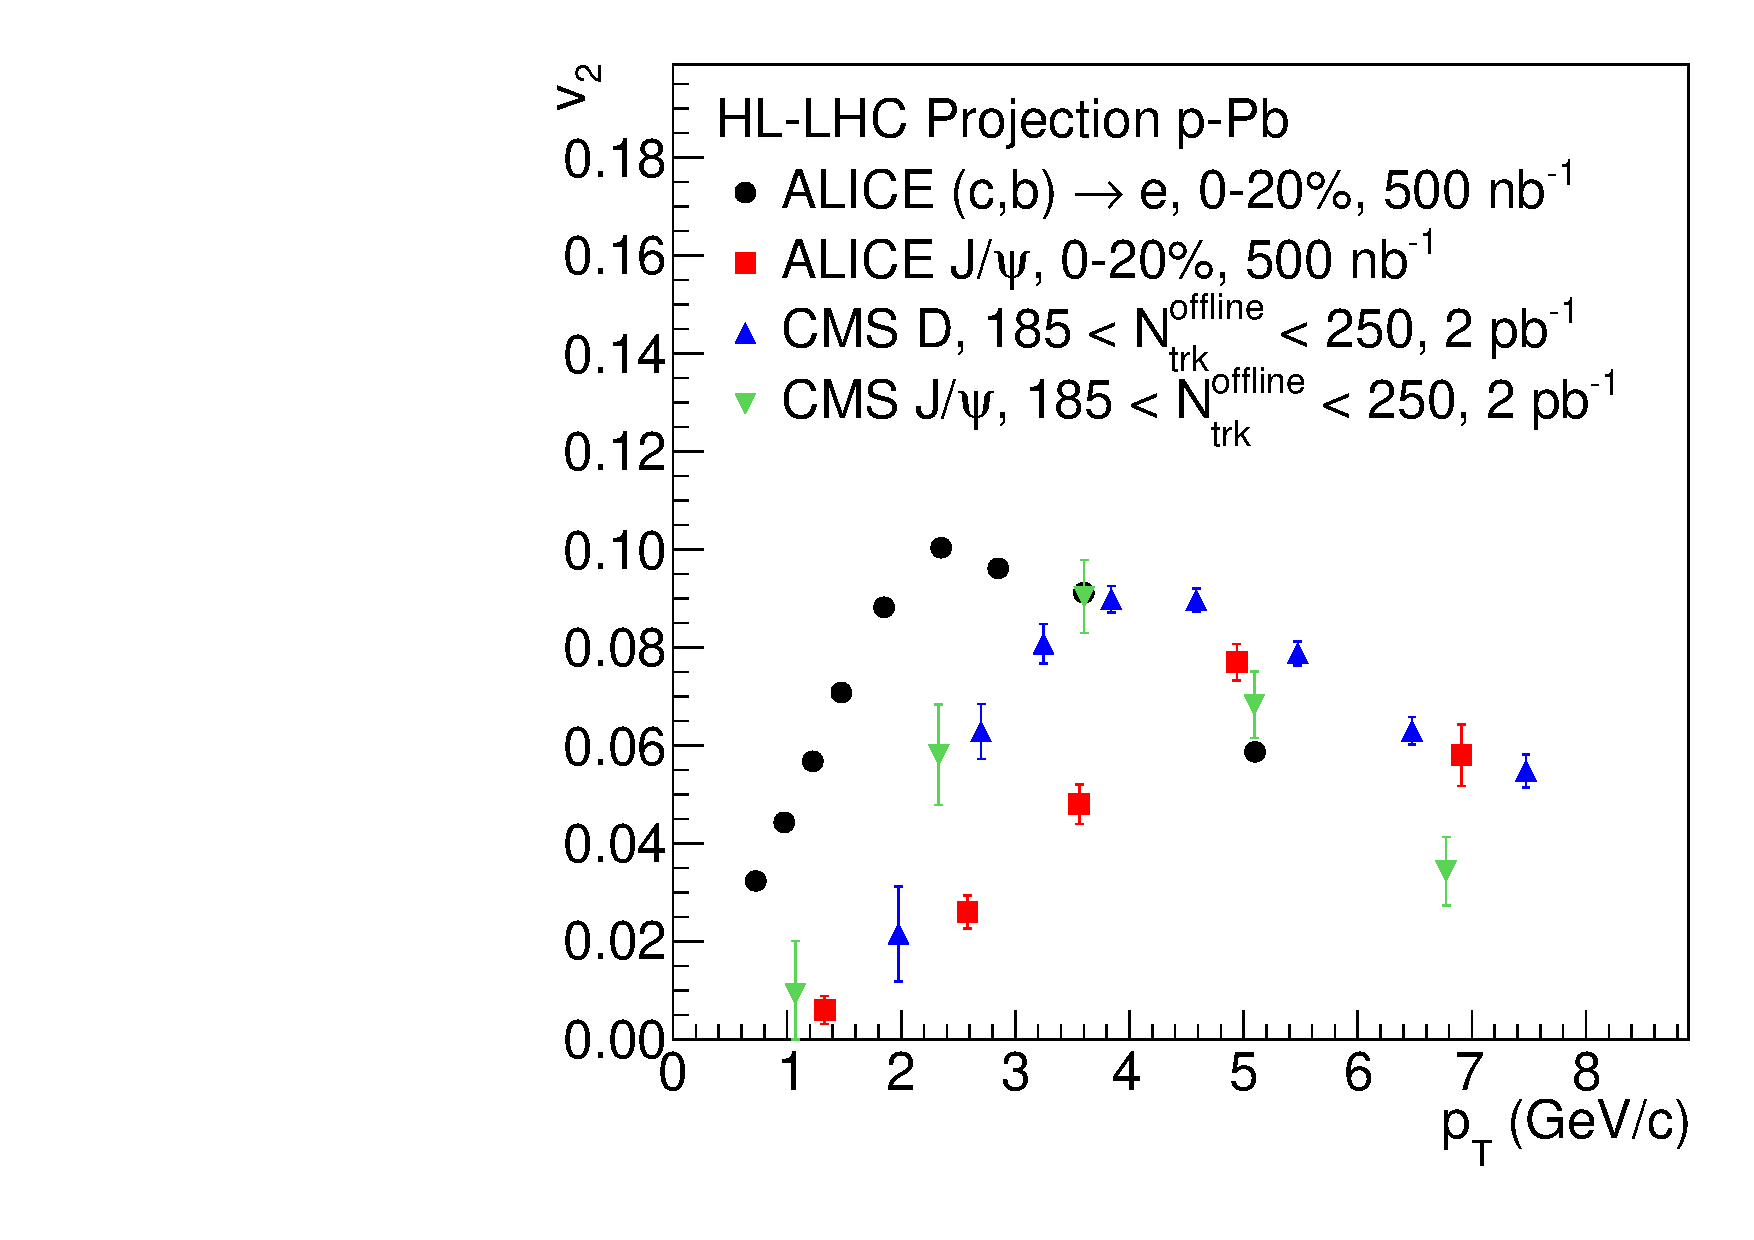
\includegraphics[width=.49\linewidth]{\main/smallsystems/img/v2_ppb.pdf}

\caption{Particle identified $v_{\rm{2}}$ coefficients for \pp (left) and \pPb collisions (right) as a function of $\pT$. In \pp... In \pPb collisions, two different cases are shown: the ALICE projections are for the 20\% highest-multiplicity collision ($L_{\rm int} = \unit[500]{nb^{-1}}$) demonstrating the negligible statistical uncertainties for heavy-flavour decay electrons and $J/\psi$, while the CMS projection is for a bin with $4-5 \nch$ ($L_{\rm int} = \unit[2]{pb^{-1}}$) demonstrating the wide reach in multiplicity achievable for $D$ mesons and $J/\psi$.
}
\label{fig:smallsystems_corr_cumulants_pid}
\end{figure}

\subsubsection{Event-by-event fluctuations of elliptic flow $\rm{p}(v_{\rm{2}})$}

The $v_{\rm{n}}$ measurements fluctuate on an event by event basis as no two nuclei have identical parton distribution. Probability density distribution, $\rm{p}(v_{\rm{n}})$ is closely related to event-by-event fluctuations of the eccentricities, $\rm{p}(\varepsilon_{\rm{n}})$. As a result, study of probability density distribution, $\rm{p}(v_{\rm{n}})$,  provides more information about the initial condition and the final state dynamics of the medium. Models predict a semi-Gaussian distribution of $\rm{p}(v_{\rm{n}})$ in large systems, while, in small systems the shape is predicted to be closer to a Gaussian. Figure~\ref{fig:smallsystems_corr_pvn} presents a projection for the measurement of $\rm{p}(v_{\rm{n}})$ in \pp collisions. This extrapolation is based on the $\rm{p}(v_{\rm{2}})$ measurement in $60-65\%$ centrality \PbPb collisions at \sqrtsNN{} 2.76 $\tev$~\cite{Aad:2013xma}. The same signal is assumed although the width of the distribution is most likely smaller in \pp collisions. Such a measurement would constitute the first measurement of $\rm{p}(v_{\rm{n}})$ in \pp collisions, and can shed important light on the nature of the observed $v_{\rm{2}}$ coefficients.

\begin{figure}[ht]
\centering
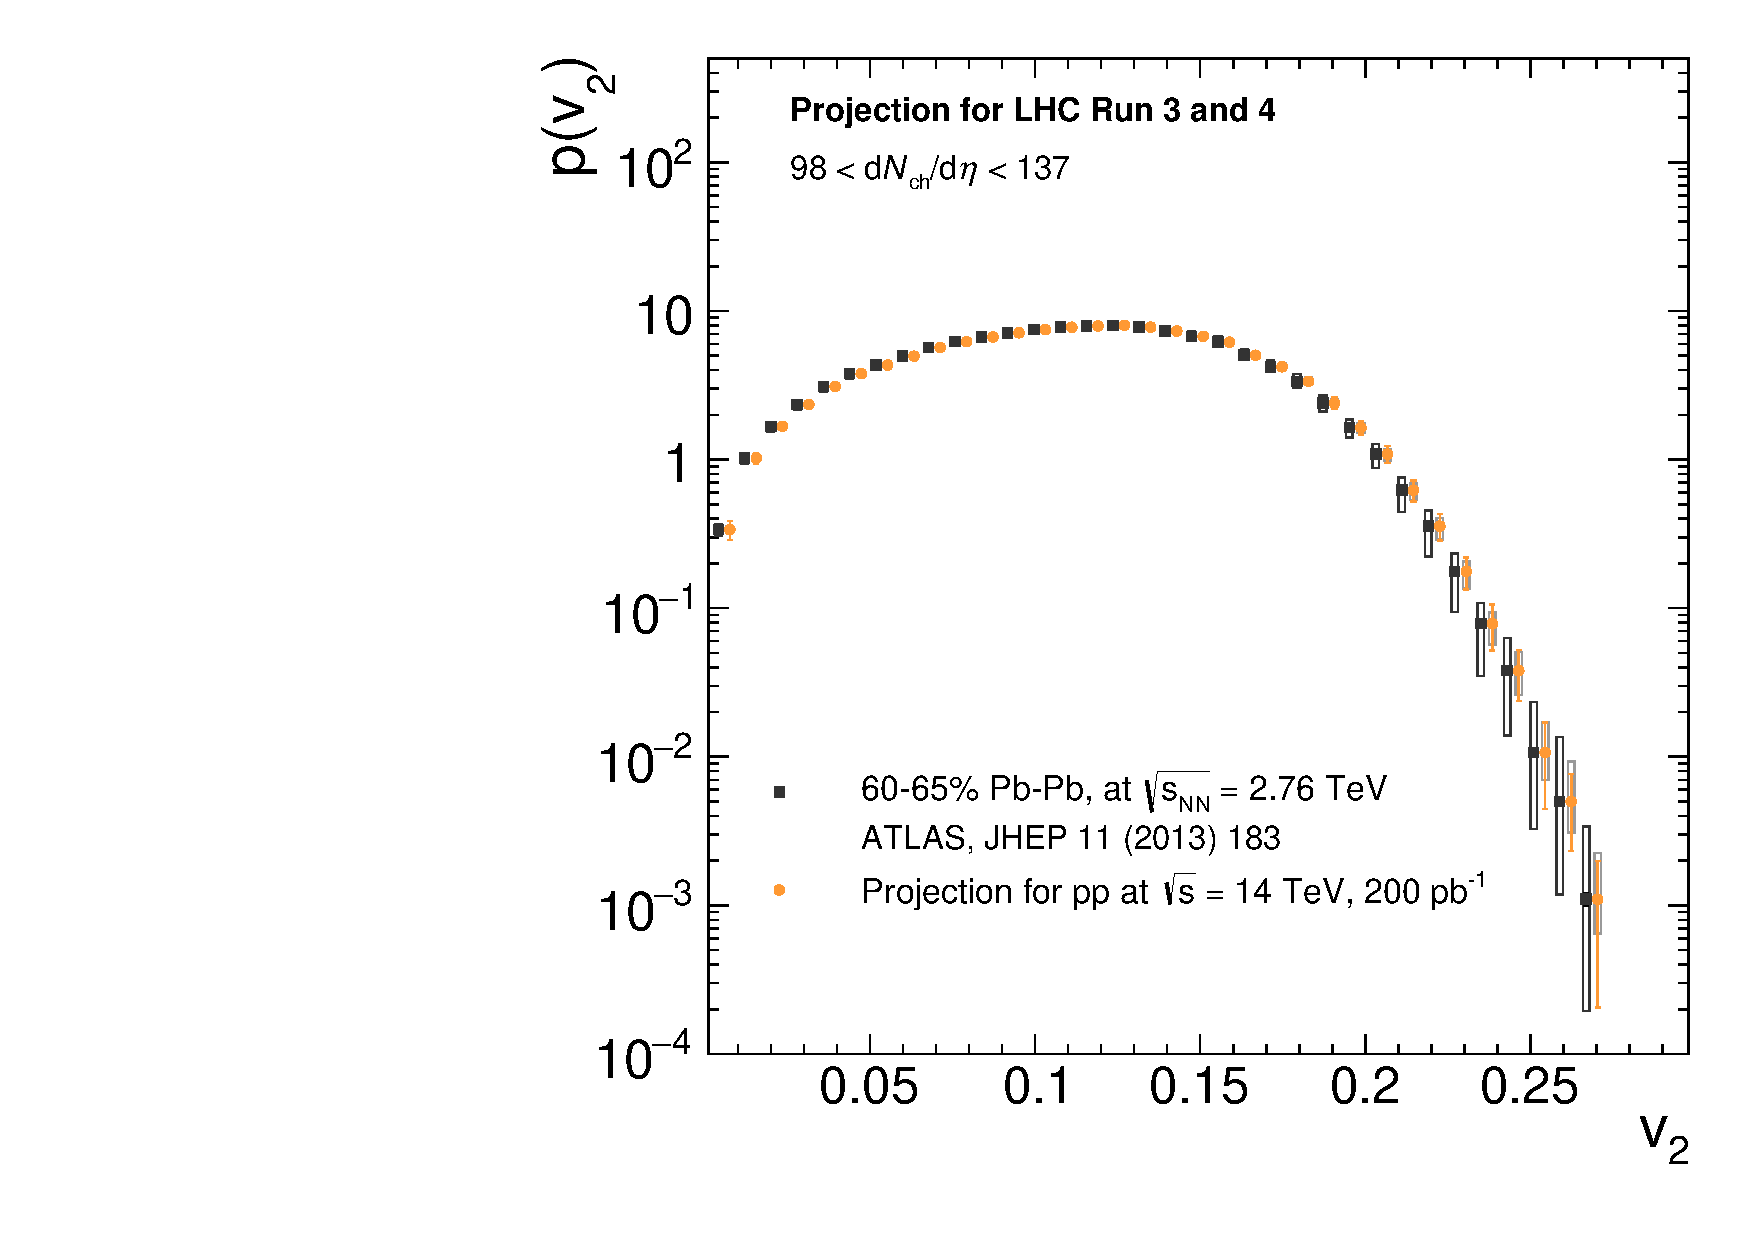
\includegraphics[width=.49\linewidth]{\main/smallsystems/img/ebye_v2_60-65_276TeVppprojection.pdf}

\caption{Projection of the measurement of the probability distribution of $v_{\rm{2}}$ in \pp collisions. To illustrate the reach the same signal as in \PbPb~\cite{Aad:2013xma} is assumed. The projection is for the equivalent \pp multiplicity (circles) to 60--65\% centrality in \PbPb collisions (squares).}
\label{fig:smallsystems_corr_pvn}
\end{figure}

\subsubsection{Strangeness Enhancement}

The unexpected increase of the strange particle yield normalized by the pion yield as a function of $\nch$ is one of the key observations in small systems. In \pp collisions these ratios are measured up to $\dNdeta \approx 17$ with some overlap with \pPb collisions. The most peripheral \PbPb collisions measured have a $\dNdeta \approx 96$. Figure~\ref{fig:smallsystems_strangeness_omega_pi} presents the expected reach of the $\Omega/\pi$ ratio in \pp collisions which will bridge the present gap between \pp and \PbPb collisions. In particular, if the measured increasing trend would continue, the $\Omega/\pi$ ratio would grow larger than in peripheral \PbPb collisions. Such an unlikely scenario will be clearly distinguishable from a scenario where the $\Omega/\pi$ flattens with increasing $\dNdeta$ and connects smoothly to \PbPb collisions. 

\begin{figure}[ht]
\centering
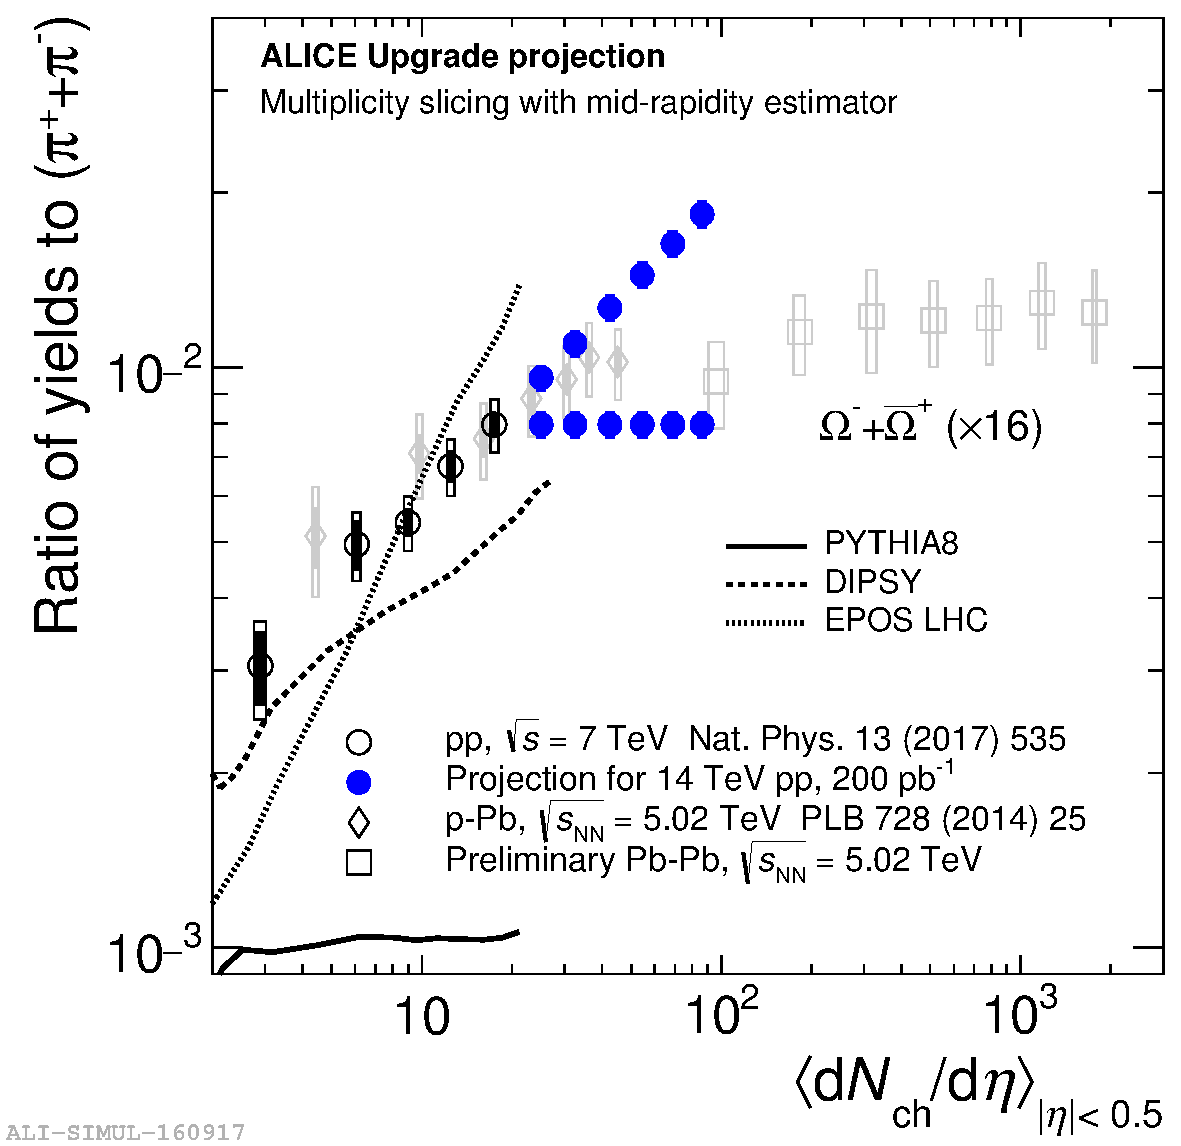
\includegraphics[width=0.49\linewidth]{\main/smallsystems/img/strangeness_omegapi.pdf}

\caption{$\Omega/\pi$ ratio as a function of $\dNdeta$ for \pp, \pPb, and \PbPb collisions. The existing data (from Ref.~\cite{ALICE:2017jyt}) is shown in open black symbols, the extrapolation for \pp collision is denoted by blue filled circles. Two scenarios are shown: a) assuming that the ratio continues increasing following the measured trend, and b) assuming that the value stays the same as at the largest measured $\dNdeta$.}
\label{fig:smallsystems_strangeness_omega_pi}
\end{figure}

\subsubsection{Energy Loss}

Narrative: 
- Existing pA eloss measurements (ALICE, ATLAS, CMS) show limit of maximal few percent quenching. In conclusion, RpA is not a good observable
- Produce estimates for a) h-jet (a la ALICE), b) gamma-jet or Z-jet (ATLAS/CMS), c) jet substructure
- Produce these for pA and pp
- For pp, see if high mu sample can be also used for something. In fact it should be made clear where it can be used and where not, as this chapter will be one of the places where a low mu pp program is motivated.

\begin{figure}[ht]
\centering
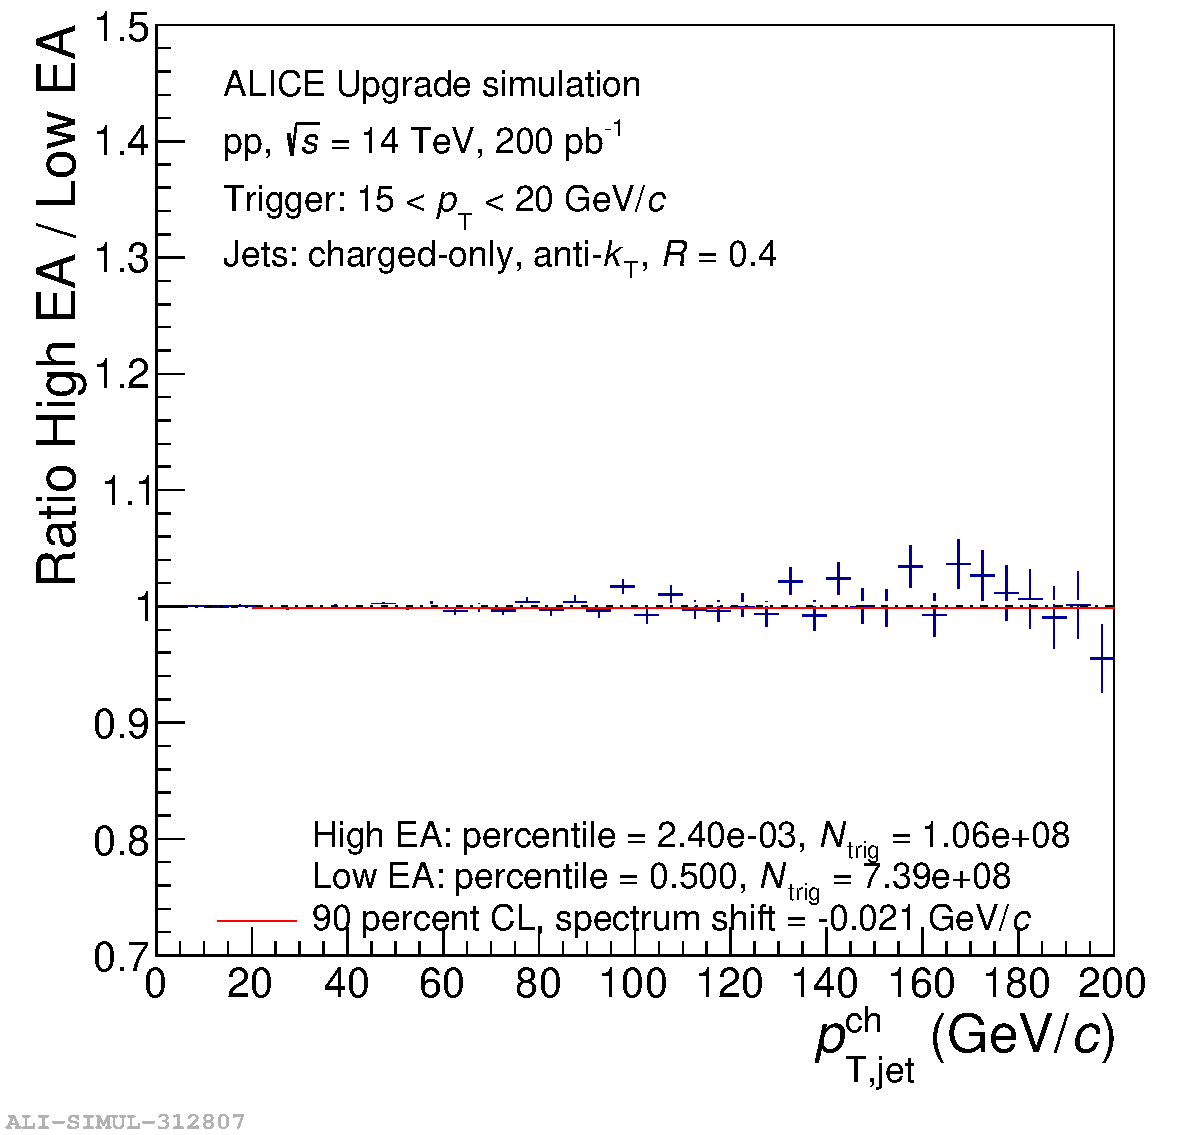
\includegraphics[width=0.49\linewidth]{\main/smallsystems/img/hjet_pp.pdf}
\hfill
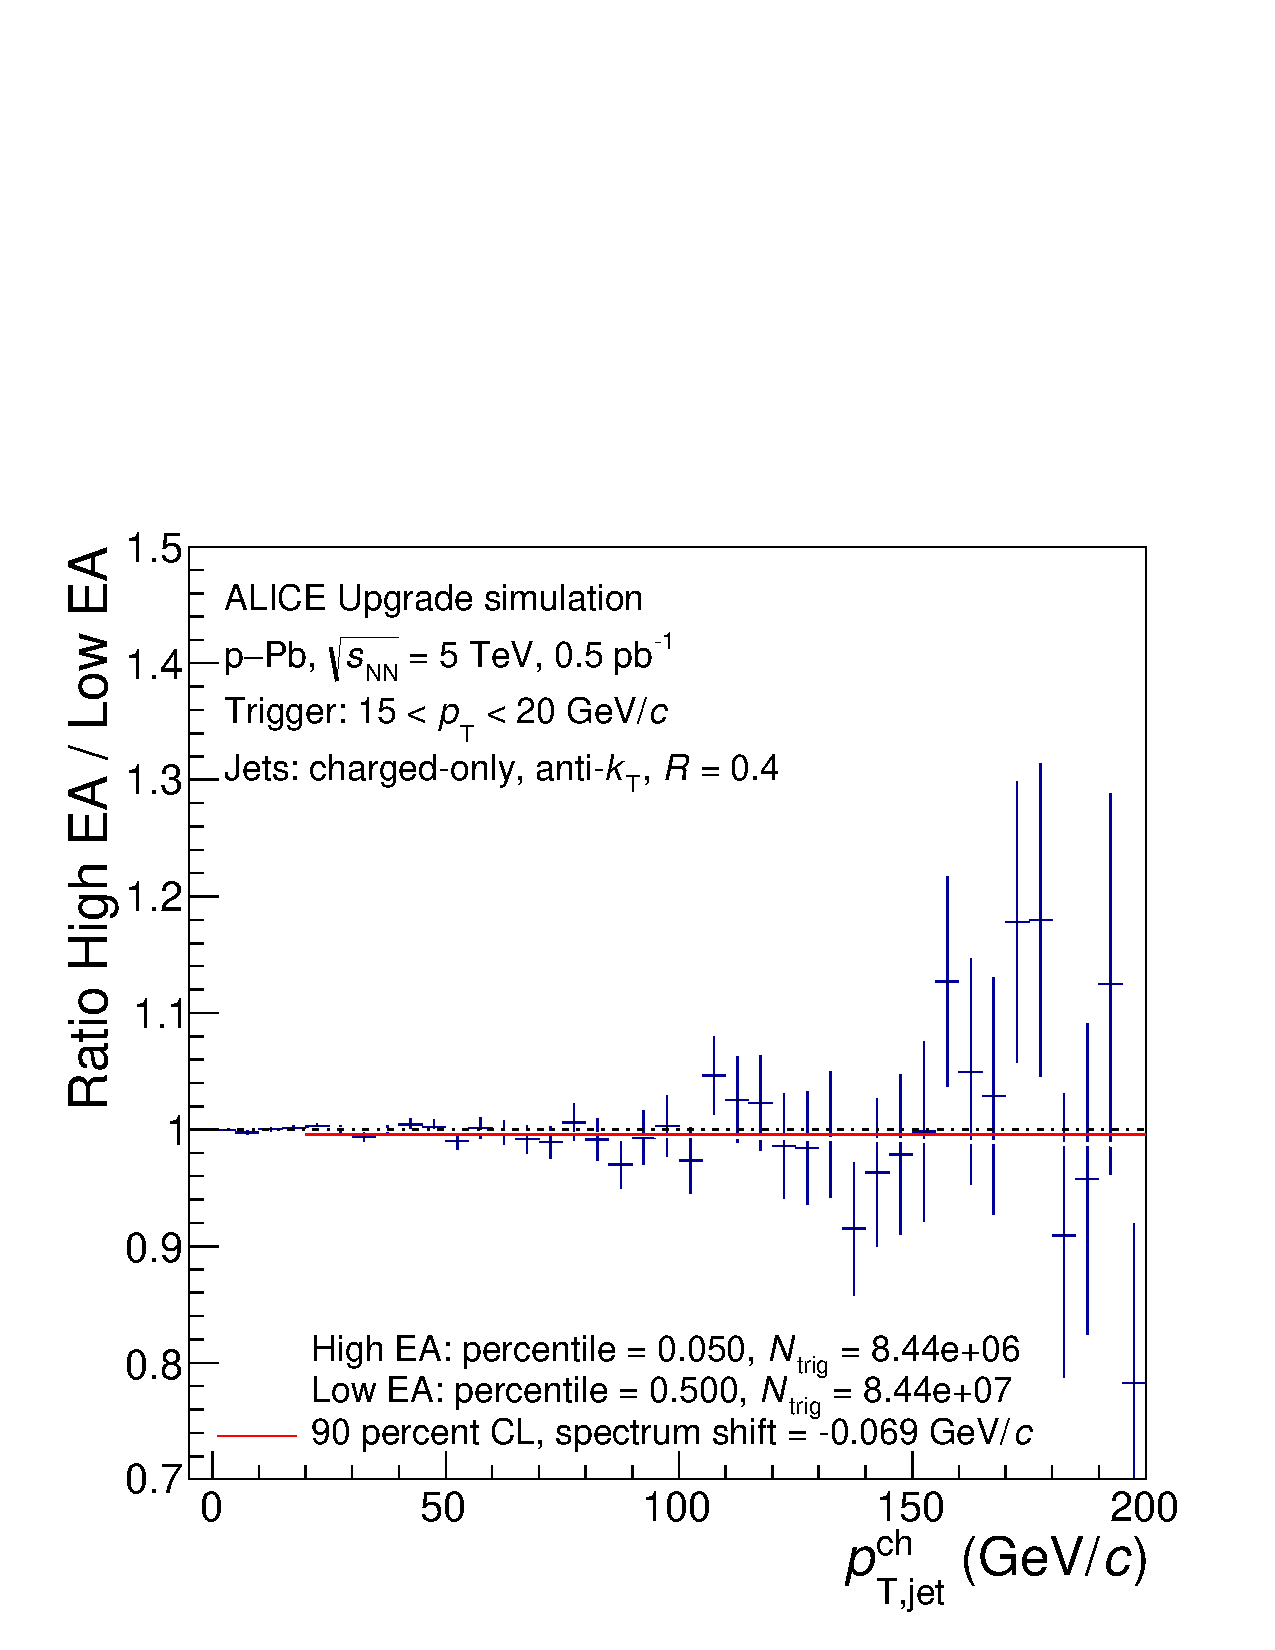
\includegraphics[width=0.49\linewidth]{\main/smallsystems/img/hjet_ppb.pdf}
\caption{Modification of jet recoil yields extracted from hadron-jet correlations for \pp collisions (left) and \pPb collisions (right). UNDER APPROVAL.}
\label{fig:smallsystems_energyloss_hjet}
\end{figure}

\begin{figure}[ht]
\centering
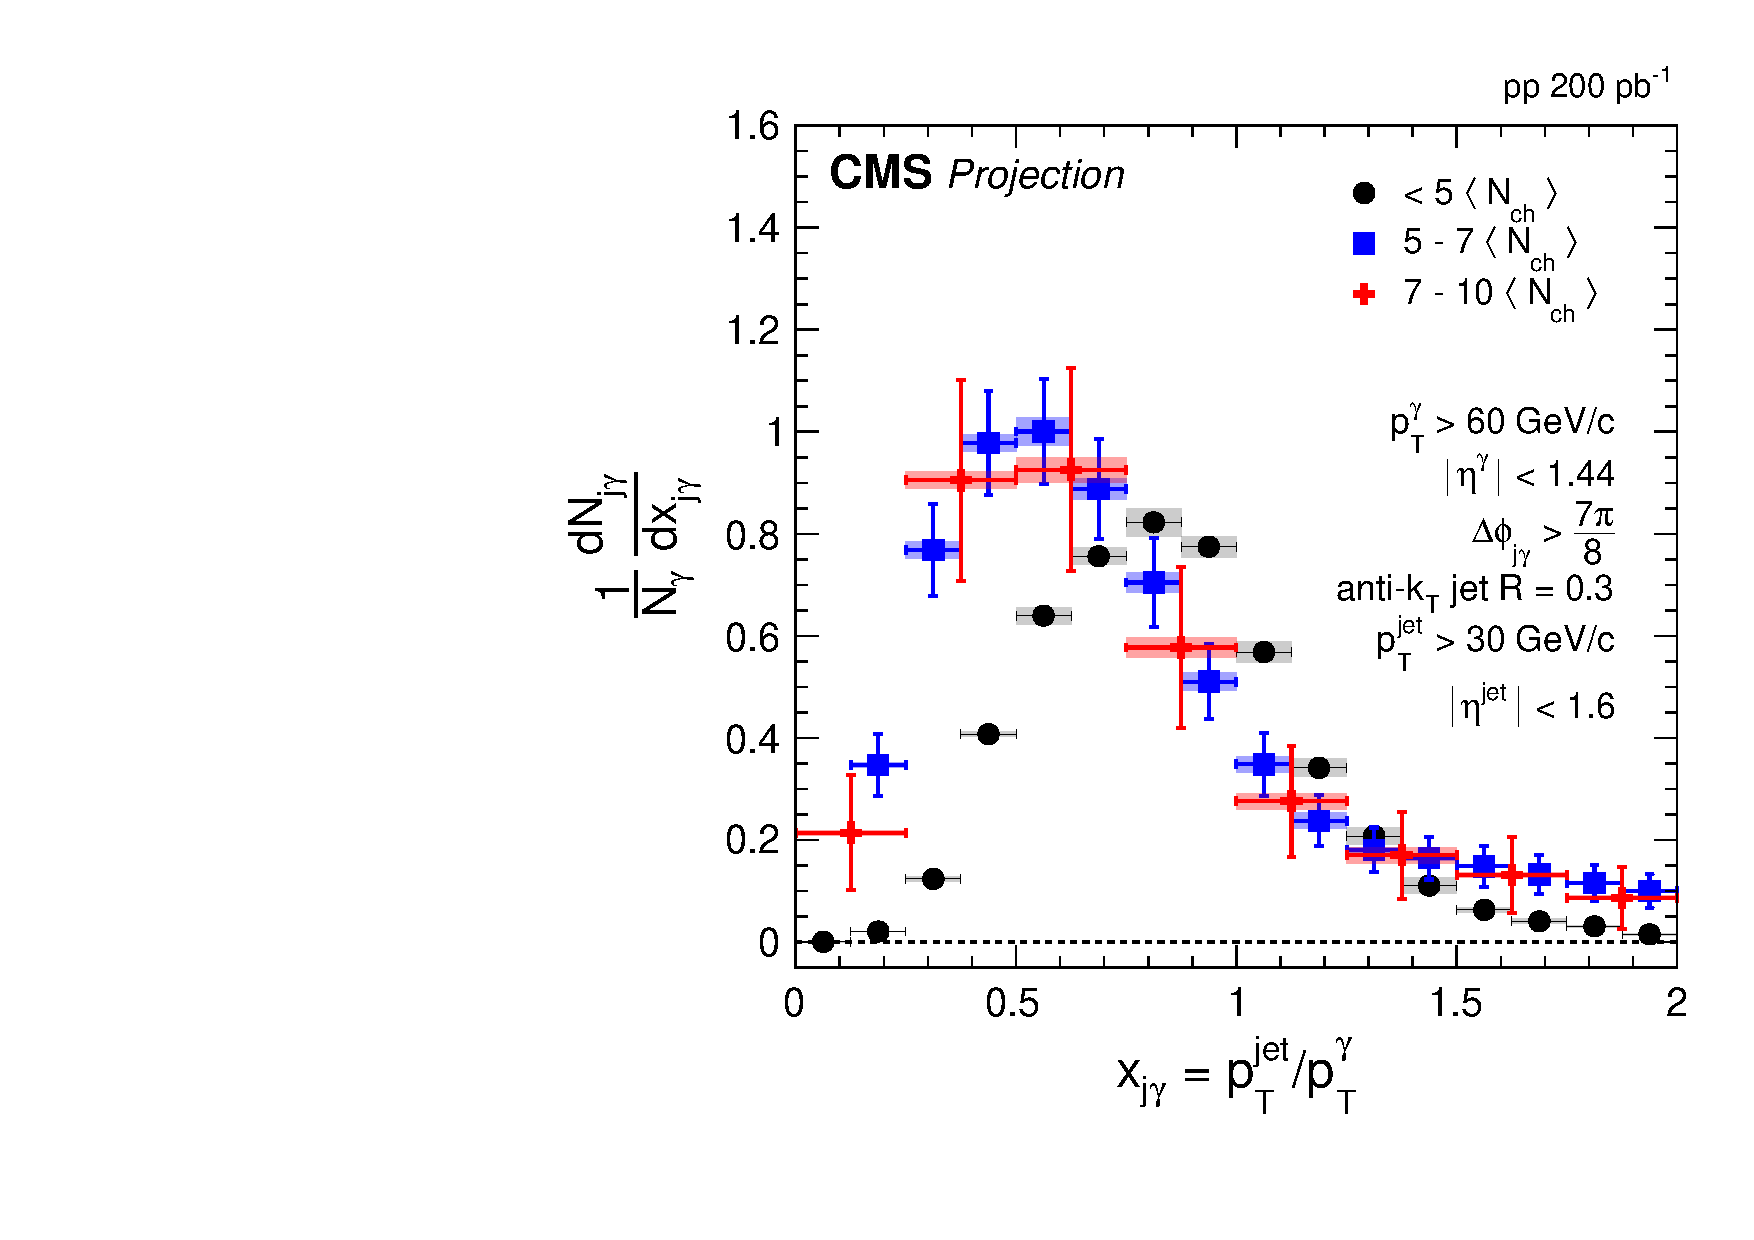
\includegraphics[width=0.49\linewidth]{\main/smallsystems/img/xjg_highmult_projection_rebin.pdf}
\hfill
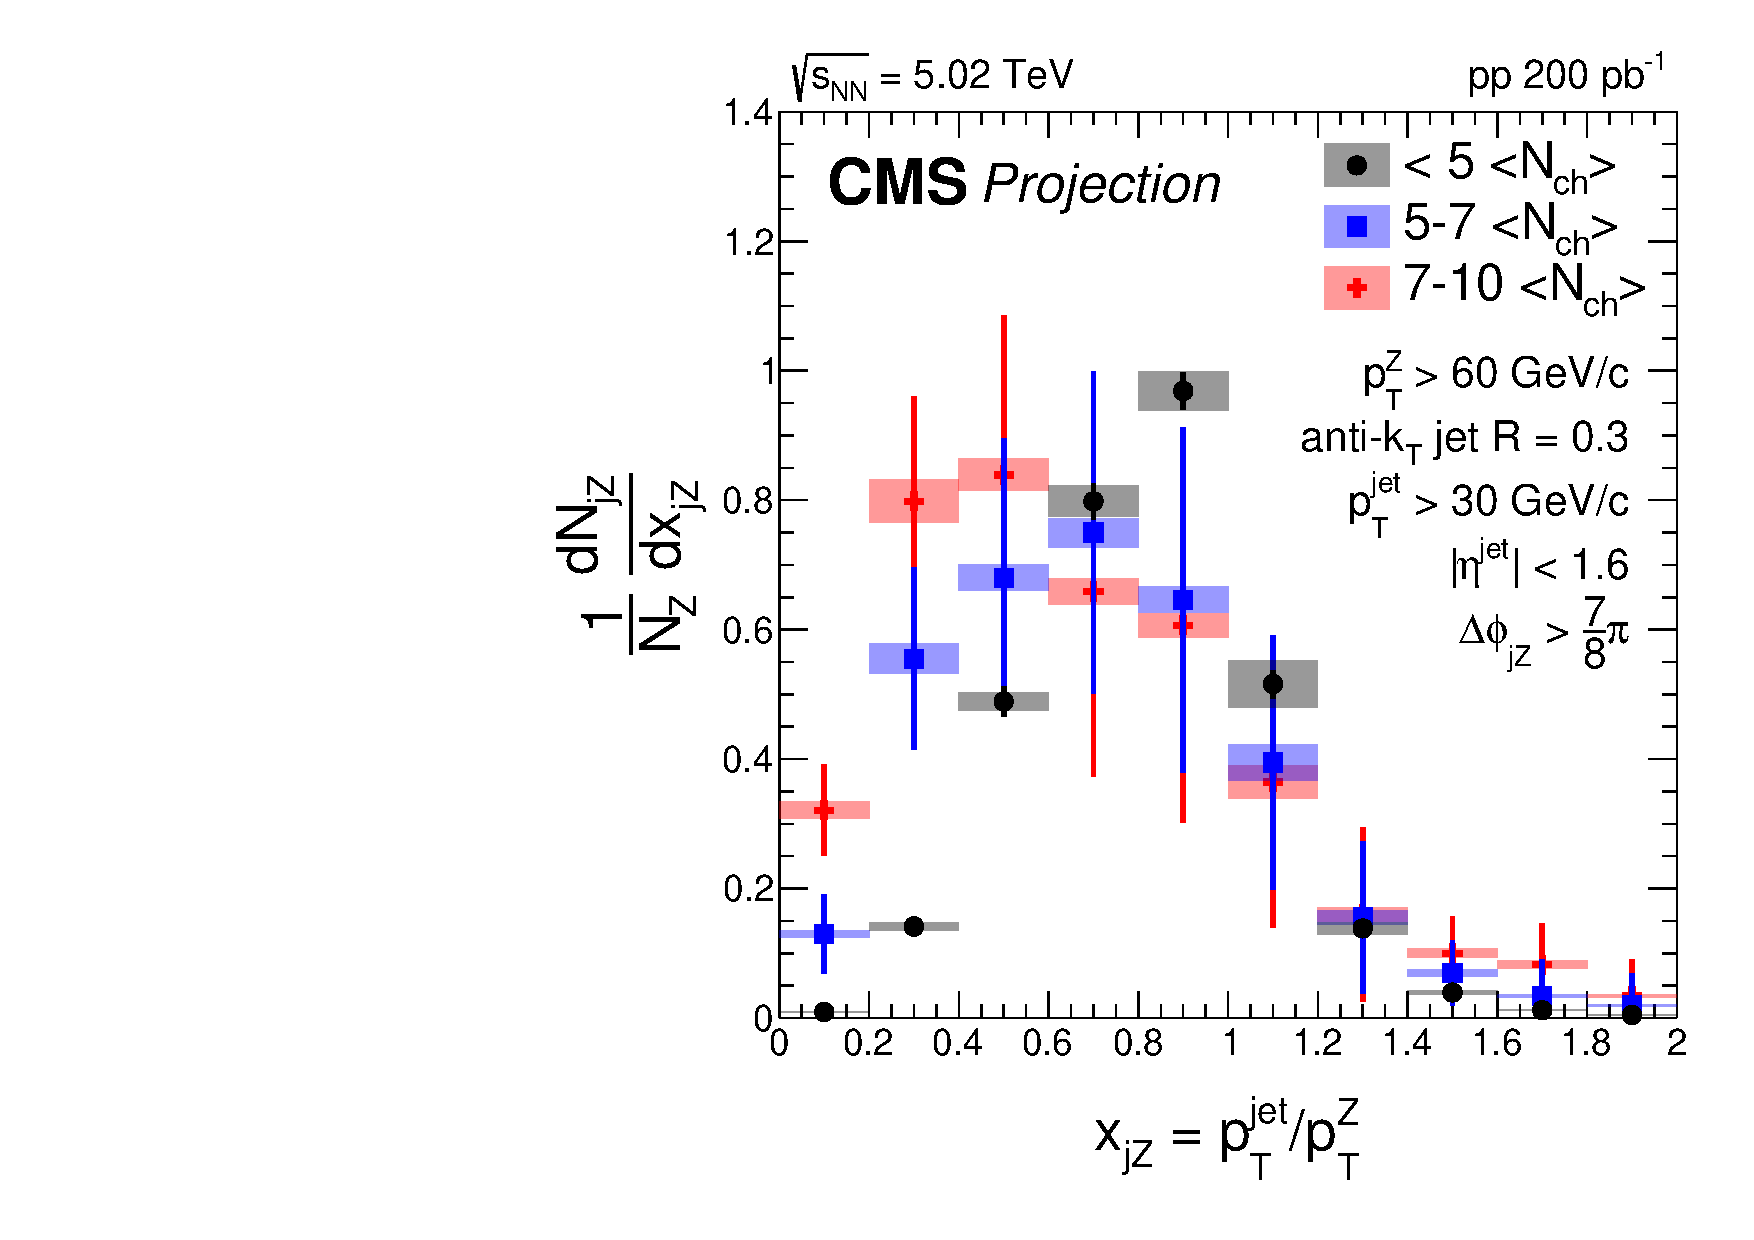
\includegraphics[width=0.49\linewidth]{\main/smallsystems/img/projection_xjz_pp_multBins.pdf}
\caption{Projections of the measurement of jet-$\gamma$ and jet-$Z$ correlations in \pp collisions. Shown are the $x_{j\gamma}$ (left panel) and $x_{jZ}$ (right panel) distributions for different multiplicity bins. The projection is based on the equivalent measurement in \pPb collisions~\cite{}. UNDER APPROVAL.} 
\label{fig:smallsystems_energyloss_xjg}
\end{figure}

\begin{figure}[ht]
\centering
\includegraphics[draft]{\main/smallsystems/img/energyloss_Zjet.pdf}

\caption{Z-jet correlations in \pp (left panel) and \pPb collisions (right panel). 1/N dN/dxZj vs xZj.}
\label{fig:smallsystems_energyloss_Zjet}
\end{figure}

\subsubsection{Thermal Radiation}

\begin{figure}[ht]
\centering
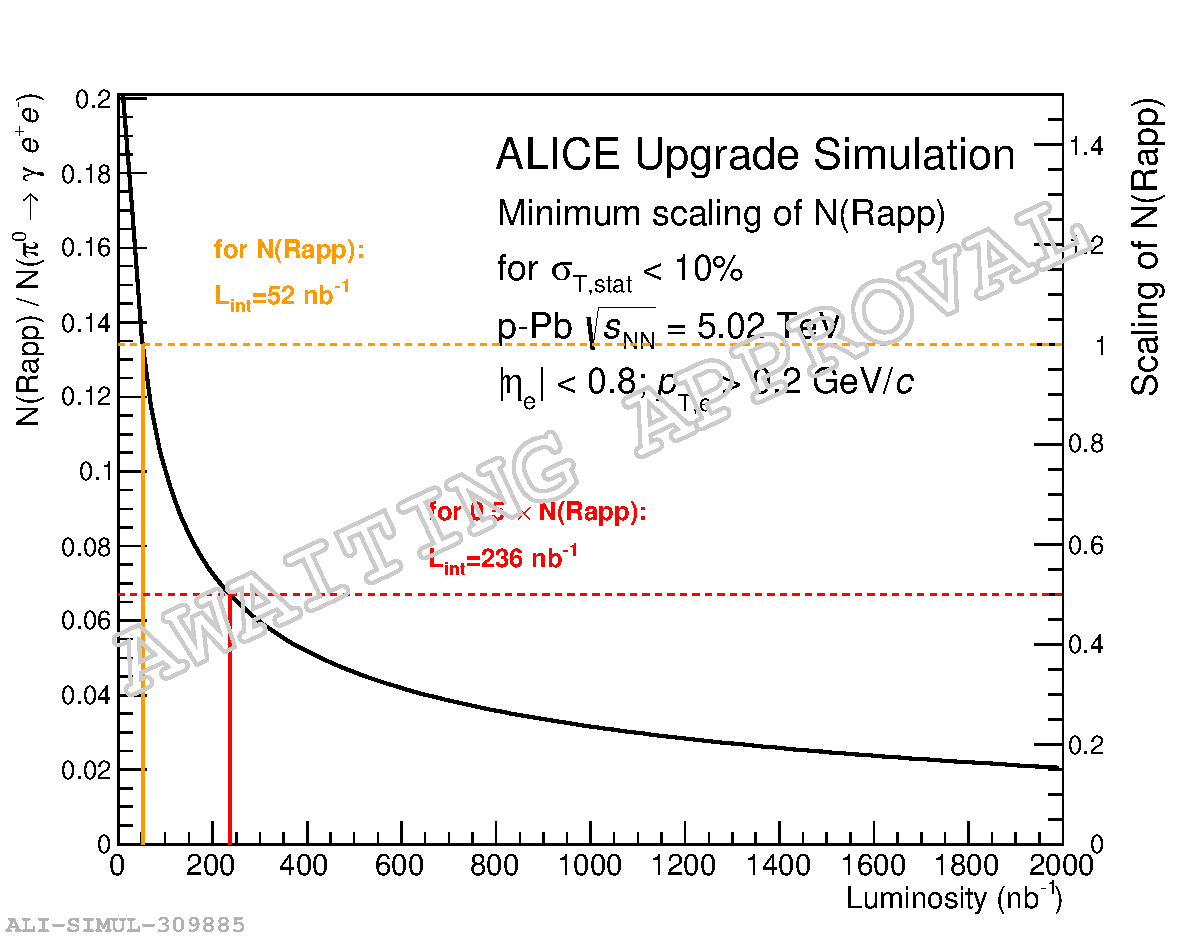
\includegraphics[width=0.7\linewidth]{\main/smallsystems/img/2018-09-29-2018-09-29-finalPlotsTemperatureComparison_pPb_FastSim_FitBG_noDCAcut_fitResults_study0.pdf}
\caption{Projection of the measurement of the medium temperature extracted from thermal dileptons in \pPb collisions. As the expected signal is uncertain, the figure presents the required integrated luminosity relative to the prediction in Ref.~\cite{}. It is expressed as the minimum thermal photon N(Rapp) to $\pi^0$ ratio (left axis) and scaling of N(Rapp) (right axis) for achieving a 10\% uncertainty on the extracted temperature.}
\label{fig:smallsystems_thermal_radition}
\end{figure}

The measurement of thermal radiation in \pPb collisions can be considered as a smoking gun for QGP formation. In order to estimate the sensitivity to the thermal radiation into the dielectron channel a similar strategy as in Sec.~\ref{sec:thermalradiation:dileptons} was used. 
The input for the signal is composed of:
\begin{itemize}
\item contributions from the decays of long-lived light pseudoscalar and vector mesons (hadronic cocktail), with particle ratios and spectral shapes extrapolated from existing heavy-ion data at lower energies,
\item correlated semileptonic charm decays based on calculations from the PYTHIA event generator \cite{Sjostrand:2006za}, 
\item and the radiation of thermal dileptons and a medium-modified spectral function for the \Prho meson in a realistic space-time evolution.
\end{itemize}
The first two are the same as for the expectations used in the extraction of dark photon limits in Sec.~\ref{sec:dileptons:darkphotons}, the latter were provided by R.~Rapp~\cite{RappPriv1}. The combinatorial background was scaled from \PbPb collisions to the expected number of pairs in \pPb collisions. The pair efficiency (including the efficiency for rejecting \Pepem pairs from semileptonic charm decays) is assumed to be the same as in \PbPb collisions. 

The temperature of the QGP is extracted in the same way as in Sec.~\ref{sec:thermalradiation:dileptons}. The minimum thermal photon to $\pi^{0}$ (both decaying into \Pepem) ratio that is needed for a fit to the invariant mass spectrum with a statistical uncertainty $\sigma_{\rm T,stat} < 10$\% as a function of integrated up to 2000 nb$^{-1}$ is shown in Fig.~\ref{fig:smallsystems_thermal_radition}. If the prediction in Ref.~\cite{RappPriv1} is accurate, an integrated luminosity of $\unit[52]{nb^{-1}}$ is sufficient. In case the real signal is 50\% smaller about 4--5 times the statistics is needed.

\subsection{Data-taking strategy}

% High multiplicity triggering, pile up, MB sample
% pp
%   ALICE: additional several month pp program
%   ATLAS/CMS: special runs (mu~1) or special conditions at end of fill
%   LHCb: either in nominal (mu~5) or special running
%   HM sample: 200 pb-1 pp (per experiment)
%   How much MB for low-multiplicity questions?
% p-Pb scheduled run
%   1000-2000 nb-1

\subsection{Summary}

\end{document}
